% main.tex -- preprint SKELETON generated from toe/TOE_ATTEMPT.md (+ CORE.md, PROOF.md, SCORECARD.md, ledger.json)
% Status: internal draft v0.6 (2026-11-07). NOT submitted, NOT published, NOT peer-reviewed.
% v0.6 folds in K4 Lean honesty (claim text only; K4 stays [P]), the Chair44 L=64 computed-diffraction hop (CH-V-020 stays [X]) and the multi-window P/F computed diffraction tables (independent of Chair44 and E_*), the already-landed L=64 q_z=0 streak image (descriptive [C on patch]), and the 2026-11-07 Solomyak [S] scope-check caveat (unique ergodicity still unverified); see CHANGES-v0.6.md.
% v0.5 closes closable prose TODOs (K4 Lean names with statement-scope caveat; [S] novelty-note scope check; Phase summaries without excluded-lineage material).
% v0.4 fills 33 previously empty ledger ids from owner-ledger-sync-2026-11-06.md (Cookies 7e6a508).
% v0.3 applies T1_scorer_robustness_2026-11-06.md preprint wording and owner-cite-todos-2026-11-06.md.
% v0.2 applies owner-first-pass-2026-11-06.md in lockstep with claims.csv and figures; see CHANGES-v0.2.md.
% v0.1 responded to referee-reports/toe-preprint-skeleton.md and novelty/theorem-F-novelty.md; see CHANGES-v0.1.md.
% Every labelled claim is defined once in claims_data.py and rendered through \useclaim{ID}.
\documentclass[11pt]{article}
\usepackage[T1]{fontenc}
\usepackage[utf8]{inputenc}
\usepackage[margin=2.3cm]{geometry}
\usepackage{amsmath,amssymb}
\usepackage[dvipsnames]{xcolor}
\usepackage{graphicx}
\usepackage{booktabs,longtable,array}
\usepackage[hidelinks]{hyperref}
% Figures: frozen v1.0 set built by the Figure Maker (no l=7 series). The build expects the
% research-publishing layout: toe-preprint/ and figures/ side by side.
\graphicspath{{../figures/proof-brackets/figs_v0.2/}{figs_v0.6/}}

% ---------- claim labels (Joey's fixed set) ----------
\makeatletter
\newcommand\defclaimcolor[2]{\expandafter\def\csname claimclr@#1\endcsname{#2}}
\defclaimcolor{P}{ForestGreen}
\defclaimcolor{C}{RoyalBlue}
\defclaimcolor{E}{BurntOrange}
\defclaimcolor{X}{Purple}
\defclaimcolor{A}{Gray}
\defclaimcolor{F}{BrickRed}
\newcommand\claimtag[1]{\ifcsname claimclr@#1\endcsname
  \fcolorbox{\csname claimclr@#1\endcsname}{\csname claimclr@#1\endcsname!12}{\sffamily\bfseries\scriptsize\textcolor{\csname claimclr@#1\endcsname}{[#1]}}%
  \else\fcolorbox{black}{white}{\sffamily\bfseries\scriptsize [#1]}\fi}
\newcommand\unverifiedtag{\,\fcolorbox{Gray}{white}{\sffamily\scriptsize\textcolor{Gray}{unverified}}}
\newcommand\pendingtag[1]{\ {\sffamily\scriptsize\textcolor{Mahogany}{[#1]}}}
% \claim[ID]{label}{text}{evidence}
\newcommand\claim[4][]{\par\smallskip\noindent\claimtag{#2}\ifx\relax#1\relax\else~{\sffamily\scriptsize\texttt{#1}}\fi\quad #3\par
  \noindent\hspace*{1.5em}{\footnotesize\textcolor{Gray}{Evidence: #4}}\par\smallskip}
\newcommand\useclaim[1]{\ifcsname claim@#1\endcsname\csname claim@#1\endcsname\else\todo{missing claim #1}\fi}
\makeatother
\newcommand\todo[1]{{\color{red}\sffamily\small[TODO: #1]}}
\newcommand\flagmark{\textsuperscript{\dag}}
% generated by build_claims.py from claims_data.py -- do not edit by hand
\expandafter\def\csname claim@S1-QIS-PNP\endcsname{\claim[S1-QIS-PNP]{F}{The QIS headline claim of an ``unconditional proof that P $\neq$ NP'' does not survive that repository's own held-out audit.}{TOE\_ATTEMPT.md \S{}8 l.401; CORE.md \S{}5 l.84; ledger.json QIS-322 [F, excluded as falsified]}}
\expandafter\def\csname claim@S1-QIS-PLANNER\endcsname{\claim[S1-QIS-PLANNER]{F}{The QIS ``64--0 planner'' record does not survive that repository's own audit.}{TOE\_ATTEMPT.md \S{}8 l.401; CORE.md \S{}5 l.84; ledger.json QIS-182 [F, excluded as falsified]}}
\expandafter\def\csname claim@K1\endcsname{\claim[K1]{P}{On a connected finite graph with $SU(2)$ links: flat $\Leftrightarrow$ gauge-trivial $\Leftrightarrow$ $\lambda_{\min}(H_U)=0$.\unverifiedtag}{CORE.md \S{}2 l.38 (source: Chair44 X1)}}
\expandafter\def\csname claim@K2\endcsname{\claim[K2]{P}{$E_* = \inf$ over finite legal patches of $\lambda^D = \lim D_R$; it depends only on the set of legal environments, is order-reversing in it, and does not depend on frequencies.\unverifiedtag}{CORE.md \S{}2 l.39 (source: XII.A)}}
\expandafter\def\csname claim@K3\endcsname{\claim[K3]{P}{Exact IMS localisation identity; $\Lambda(\chi)\le E_*\le D_R$ with $D_R-\Lambda\le\varepsilon(\chi)$; rate $R^{-2}$ on doubling or Euclidean graphs, and $R^{-2}$ is optimal; property A alone gives no power law (lamplighter).\unverifiedtag}{CORE.md \S{}2 l.40 (source: XII.B, XII.C)}}
\expandafter\def\csname claim@K4\endcsname{\claim[K4]{P}{Every geometry-compatible frame field has $\ge 12$ of the 21 centre-octant two-cycles non-trivial in every level-1 supertile, so the connection is never pure gauge. Lean kernel-checks only encoded finite predicates; this geometric statement is not itself a kernel-checked Lean theorem.}{CORE.md \S{}2 l.41 (source: Phase VII-B P1)}}
\expandafter\def\csname claim@K5\endcsname{\claim[K5]{C}{$E_*>0$ $\Leftrightarrow$ some $T_k$ is not flat. All 1098 gauge classes of the 6561 proper rules have $E_*\ge 3.788$.}{CORE.md \S{}2 l.42 (source: X3)}}
\expandafter\def\csname claim@K6\endcsname{\claim[K6]{C}{No lower bound on $E_*$ follows from plaquette-class frequencies: there are two $\mathbb{Z}^3$ connections with the same $Q_8$ class on every plaquette and floors separated by $\ge 0.18$.\unverifiedtag}{CORE.md \S{}2 l.43 (source: X4, X5, XII.P63); source label [P/C]}}
\expandafter\def\csname claim@K7\endcsname{\claim[K7]{P}{The non-spinor floors are functions of the plaquette class field; the X.5 separation lives in the spinor component.\unverifiedtag}{CORE.md \S{}2 l.44 (source: XI.H3)}}
\expandafter\def\csname claim@K8\endcsname{\claim[K8]{P}{Orbit Lemma: $\sigma_{dQ}=\rho_Q\circ\sigma_d$, $\rho_Q$ is a global gauge transformation, $T_1(dQ)\cong T_1(d)$, and $E_*(dQ)=E_*(d)$ on the conjugation stabiliser; outside it the equivalence can fail from level 2.\unverifiedtag}{CORE.md \S{}2 l.45 (source: XII.OL)}}
\expandafter\def\csname claim@K9\endcsname{\claim[K9]{C}{$E_*(1387)\in[9.1104981,\,9.3616608]$; $E_*(539311)\in[9.2083494,\,9.3817818]$; the maximiser over all $6^8$ rules is one of 1387, 539311, 539291.}{CORE.md \S{}2 l.46 (source: XII.R20, XII.r24, XII.F4)}}
\expandafter\def\csname claim@K10\endcsname{\claim[K10]{C}{No function of level-one data determines $E_*$ (1387 against 539288).\unverifiedtag}{CORE.md \S{}2 l.47 (source: XII.T31); source label [P+C]}}
\expandafter\def\csname claim@K11\endcsname{\claim[K11]{P}{For every $Q_8$ gauge section $s$ of a patch $K$: $\lambda_{\min}(P_KHP_K)\le B(s)=[\sum_e(2-2\,\mathrm{Re}\,d_e)+b(K)]/|K|$; the floor is bounded by the unique-games frustration energy of any section.\unverifiedtag}{CORE.md \S{}2 l.48 (source: XII.ug.P151)}}
\expandafter\def\csname claim@K12\endcsname{\claim[K12]{P}{The Clifford transports lie in $Q_8$; on vectors (the adjoint) the link group is the Klein group $V_4$; in two dimensions the Pauli-frame connections are $\mathbb{Z}_4$-valued (Abelian).\unverifiedtag}{CORE.md \S{}2 l.49 (source: CLIFFORD\_Q8\_PHASE2 Thms 2.2-2.3; X6)}}
\expandafter\def\csname claim@K13\endcsname{\claim[K13]{P}{No chirality: Wilson traces and plaquette classes are identical for a tiling and its mirror.\unverifiedtag}{CORE.md \S{}2 l.50 (source: CLIFFORD\_Q8\_PHASE2 Thm 2.4)}}
\expandafter\def\csname claim@K14\endcsname{\claim[K14]{P}{Diamagnetic bound: $\lambda_{\min}(H_U)\ge\lambda_{\min}(H_1)$ on every patch, for every unitary connection (Kato's inequality; standard).\unverifiedtag}{CORE.md \S{}2 l.51 (source: standard; prereg/G1\_volume\_scaling.json T1)}}
\expandafter\def\csname claim@K15\endcsname{\claim[K15]{P}{In infinite volume, independent ($\beta=0$) links, and every finite-$\beta$ Gibbs measure of a finite-group Wilson action, give floor 0 almost surely (finite energy plus Borel--Cantelli).\unverifiedtag}{CORE.md \S{}2 l.52 (source: Phase VII \S{}8; prereg/G1\_volume\_scaling.json T3)}}
\expandafter\def\csname claim@I-TSEITIN\endcsname{\claim[I-TSEITIN]{P}{Tseitin parity formulas are unsatisfiable iff the total charge is odd ($\mathbf{1}_V\in\ker$ of the incidence over $\mathbb{F}_2$); this is the $\mathbb{Z}_2$ coboundary side of the core, in transposed form.\unverifiedtag}{TOE\_ATTEMPT.md \S{}2 l.63; CORE.md \S{}3 l.61}}
\expandafter\def\csname claim@I-ENERGY\endcsname{\claim[I-ENERGY]{P}{The continuous multilinear energy of a Tseitin instance has floor $E_{\min}\ge 1$.\unverifiedtag}{CORE.md \S{}3 l.62}}
\expandafter\def\csname claim@I-ENERGY-INST\endcsname{\claim[I-ENERGY-INST]{A}{Read as an instance of the core, that floor is an analogy only: it is the floor of a relaxation energy, not of a covariant Laplacian.}{CORE.md \S{}3 l.62}}
\expandafter\def\csname claim@I-XIII-SCOPE\endcsname{\claim[I-XIII-SCOPE]{P}{Scope statement: unique-games instances with $G=Q_8$ are the combinatorial side of the core; the external Unique Games Theorem is worst-case on finite instances and bounds no floor. (The external theorem itself is not checked here.)\unverifiedtag}{TOE\_ATTEMPT.md \S{}2 l.64; CORE.md \S{}3 l.60}}
\expandafter\def\csname claim@I-UG-EXT\endcsname{\claim[I-UG-EXT]{X}{Third-party claims (Unique Games Theorem / Min-UnCut hardness; ``Family 378: ETH is false'') are recorded as external and unchecked.}{CORE.md \S{}3 l.69}}
\expandafter\def\csname claim@I-QIS320\endcsname{\claim[I-QIS320]{E}{The Laplacian $\lambda_2$ of SAT clause graphs plateaus near $1.01$ as $N$ grows.}{CORE.md \S{}3 l.64; ledger.json QIS-320}\footnote{\textbf{Flag (I-QIS320):} ledger QIS-320 label E; source\_label 'certified' (ledger did not upgrade)}}
\expandafter\def\csname claim@I-QIS320-INST\endcsname{\claim[I-QIS320-INST]{A}{As an instance of the core this is an analogy only: a scalar (trivial-representation) graph Laplacian with no connection.}{CORE.md \S{}3 l.64; \S{}5 l.87}}
\expandafter\def\csname claim@I-QIS299\endcsname{\claim[I-QIS299]{F}{``Residual frustrated clauses carry a non-trivial 1-cycle'' (a would-be holonomy statement for a $\mathbb{Z}_2/\mathbb{R}$ cochain) is falsified.}{CORE.md \S{}3 l.65; ledger.json QIS-299}}
\expandafter\def\csname claim@I-GU-C4\endcsname{\claim[I-GU-C4]{C}{The 4D chair $C_4$ has face counts $(80,212,210,92,15)$, $\chi=1$; its boundary has $(80,208,192,64)$, $\chi=0$ (geometry only; no connection).}{CORE.md \S{}3 l.67; ledger.json GU-001}}
\expandafter\def\csname claim@I-GU-A\endcsname{\claim[I-GU-A]{A}{Geometric Unity: the fibre of $\mathrm{Met}(X)$ as an internal space is a structural analogy only (no shared object).}{CORE.md \S{}3 l.68}}
\expandafter\def\csname claim@I-WOLFRAM\endcsname{\claim[I-WOLFRAM]{A}{Hypergraph rewriting (Wolfram Physics Project) is substitution-like rewriting of graphs with no group-valued connection on a fixed substitution hull: analogy only.}{CORE.md \S{}3 l.70}}
\expandafter\def\csname claim@I-XIV-H1\endcsname{\claim[I-XIV-H1]{F}{Phase XIV (dynamical $Q_8$ Wilson ensemble) prediction H1: the hot-series $\langle\lambda_{\min}\rangle(\beta)$ is non-increasing within 3\,SE --- falsified.}{CORE.md \S{}3 l.59; TOE\_ATTEMPT.md \S{}4 row 8 l.319; ledger.json CH14-XIV.H1}}
\expandafter\def\csname claim@I-XIV-H2\endcsname{\claim[I-XIV-H2]{F}{Phase XIV prediction H2: $Y_3(1387)$ exceeds every sampled $\lambda_{\min}$ at every $\beta$ --- falsified.}{CORE.md \S{}3 l.59; TOE\_ATTEMPT.md \S{}4 row 8 l.319; ledger.json CH14-XIV.H2}}
\expandafter\def\csname claim@I-XIV-H3\endcsname{\claim[I-XIV-H3]{E}{Phase XIV H3 holds: the floor falls fastest where the inter-tile plaquette rises fastest (within one grid step).}{CORE.md \S{}3 l.59; ledger.json CH14-XIV.H3}}
\expandafter\def\csname claim@I-VI-017\endcsname{\claim[I-VI-017]{F}{The earlier (Phase VI) claim that random i.i.d.\ $Q_8$ links are gapped (floor $\approx 14.4$) is withdrawn/falsified; G1 explains it as a pre-asymptotic plateau.}{TOE\_ATTEMPT.md \S{}3.1 l.115; ledger.json CH-VI-017}}
\expandafter\def\csname claim@G1-T1\endcsname{\claim[G1-T1]{P}{T1: the diamagnetic bound and compression give $\lambda_1(T_L)\le\lambda(T_L)\le\min$ over the eight child supertiles.\unverifiedtag}{TOE\_ATTEMPT.md \S{}3.1 l.90}}
\expandafter\def\csname claim@G1-T2\endcsname{\claim[G1-T2]{P}{T2: the children are i.i.d.\ copies of $T_{L-1}$, so $P(\lambda(T_L)>x)\le P(\lambda(T_{L-1})>x)^8$.\unverifiedtag}{TOE\_ATTEMPT.md \S{}3.1 l.91}}
\expandafter\def\csname claim@G1-T3\endcsname{\claim[G1-T3]{P}{T3: for every $\beta\in[0,\infty)$ and every infinite-volume Gibbs measure of a finite-group Wilson action on the hull, $\inf\sigma(H_U)=0$ almost surely (standard argument; not claimed new).\unverifiedtag}{TOE\_ATTEMPT.md \S{}3.1 l.92-94; ledger.json TOE-G1-T3}\footnote{\textbf{Flag (G1-T3):} ledger evidence cites stale 'TOE\_ATTEMPT.md s4.1' (now \S{}3.1)}}
\expandafter\def\csname claim@G1-RARE\endcsname{\claim[G1-RARE]{X}{Rare-region scale: a trivial 1-star has probability $8^{-24}\approx 2\cdot10^{-22}$ at $\beta=0$, so the regions that drive the floor to 0 first appear at about $10^{22}$ tiles, far beyond $T_5$.\pendingtag{label pending author ruling on 'P-level estimate'}}{TOE\_ATTEMPT.md \S{}3.1 l.95; source label [P-level estimate]}\footnote{\textbf{Flag (G1-RARE):} non-standard source label 'P-level estimate'; printed [X] pending ruling}}
\expandafter\def\csname claim@G1-FLOORS\endcsname{\claim[G1-FLOORS]{E}{$Q_8$ mean floors on $T_1\ldots T_5$ ($\beta=0$, 2780 samples): 18.511, 16.024, 15.036, 14.615, 14.367 ($\pm$0.027, 0.015, 0.009, 0.008, 0.014).}{TOE\_ATTEMPT.md \S{}3.1 l.98; results/g1\_score.json}}
\expandafter\def\csname claim@G1-TRIVIAL\endcsname{\claim[G1-TRIVIAL]{E}{The trivial-connection floor falls from 11.21 to 0.139 over $T_1\ldots T_5$.}{TOE\_ATTEMPT.md \S{}3.1 l.99}}
\expandafter\def\csname claim@TOE-G1-T1\endcsname{\claim[TOE-G1-T1]{E}{Every $\beta=0$ sample obeys T1 (0 violations).}{TOE\_ATTEMPT.md \S{}3.1 l.100; ledger.json TOE-G1-T1 [C]}\footnote{\textbf{Flag (TOE-G1-T1):} LABEL MISMATCH: TOE\_ATTEMPT lists this under 'Results [E, simulated]', ledger says [C]; weaker [E] used (no upgrade); needs ledger reconciliation}}
\expandafter\def\csname claim@TOE-G1-T2\endcsname{\claim[TOE-G1-T2]{E}{T2 holds at every level: mean $\beta=0$ floor of $T_L\le E[\min$ of 8 i.i.d.\ level-$(L-1)$ floors$]+3$\,SE, $L=2..5$.}{TOE\_ATTEMPT.md \S{}3.1 l.100; ledger.json TOE-G1-T2}}
\expandafter\def\csname claim@TOE-G1-H1\endcsname{\claim[TOE-G1-H1]{F}{H1 (preregistered): the ground state sits (weight $\ge\frac12$) on the weakest child in $\ge 2/3$ of samples. Outcome: fractions 0.345, 0.450, 0.650 ($L=3,4,5$).}{TOE\_ATTEMPT.md \S{}3.1 l.106; ledger.json TOE-G1-H1}}
\expandafter\def\csname claim@TOE-G1-H2\endcsname{\claim[TOE-G1-H2]{F}{H2 (preregistered): min-stable median law $\hat m$ = 0.0830-quantile of level $L-1$. Outcome: medians below the band at $L=3,4$, inside at $L=5$.}{TOE\_ATTEMPT.md \S{}3.1 l.107; ledger.json TOE-G1-H2}}
\expandafter\def\csname claim@TOE-G1-H3a\endcsname{\claim[TOE-G1-H3a]{E}{H3a holds: $2I$ and $SU(2)$ floors agree within $3\sigma$ ($\Delta=+0.016,-0.006,+0.024$).}{TOE\_ATTEMPT.md \S{}3.1 l.108; ledger.json TOE-G1-H3a}}
\expandafter\def\csname claim@TOE-G1-H3b\endcsname{\claim[TOE-G1-H3b]{F}{H3b (preregistered): $Q_8$ significantly below $SU(2)$. Outcome: right sign ($-0.021,-0.014,-0.017$) but never beyond $3\sigma$.}{TOE\_ATTEMPT.md \S{}3.1 l.109; ledger.json TOE-G1-H3b}}
\expandafter\def\csname claim@TOE-G1-H4\endcsname{\claim[TOE-G1-H4]{E}{H4 holds (weak test, recorded as such): medians (18.53 \ldots 14.39) lie above the certified $E_*(1387)\ge 9.1104981$.}{TOE\_ATTEMPT.md \S{}3.1 l.110; ledger.json TOE-G1-H4}}
\expandafter\def\csname claim@SC-8\endcsname{\claim[SC-8]{P}{Scorecard row 8 (programme-internal), settled negatively: in infinite volume the matter floor is 0 at every $\beta$ for finite groups (G1 T3), so it is not an infinite-volume order parameter of any finite-group Wilson ensemble.\unverifiedtag}{TOE\_ATTEMPT.md \S{}3.1 l.116; \S{}4 row 8 l.319}\footnote{\textbf{Flag (SC-8):} README.md says 'One scorecard row is [P]' but row 8 is '[P] negative' (discrepancies.md \S{}2.7)}}
\expandafter\def\csname claim@G2B-DERIV\endcsname{\claim[G2B-DERIV]{E}{Derivation: $\lambda(T_L,\theta)=\lambda_1(T_L)+c_L\theta^2+O(\theta^3)$, with $c_L$ = dia $-$ para given exactly by second-order perturbation theory about the Dirichlet ground state.\pendingtag{label pending author ruling on 'P-level'}}{TOE\_ATTEMPT.md \S{}3.2 l.129; source label [P-level]}\footnote{\textbf{Flag (G2B-DERIV):} non-standard source label 'P-level'; printed [E] pending ruling; the proved version is TOE-PROOF-A}}
\expandafter\def\csname claim@G2B-CL\endcsname{\claim[G2B-CL]{E}{Floating-point $c_L$: FR30 $8.704, 11.324, 12.674, 13.046, 13.243, 13.318$; 1387 $9.850, 12.458, 13.685, 14.039, 14.196, 14.253$; $G_6/(\pi^2c_6)=0.9992$ for both. The frozen B2 geometric extrapolation from $(c_4,c_5,c_6)$ gives $c_\infty\approx13.364$ (FR30), $14.285$ (1387); from $(c_3,c_4,c_5)$ the same formula gives $13.463$ and $14.322$ (four-decimal inputs), so the extrapolated value moves by $0.10$ and $0.04$ with the fitting range. The geometric model $c_L=c_\infty-Aq^L$ has three parameters and is fitted to three points exactly, so no goodness-of-fit statistic exists; the range sensitivity is the only check. Both lie inside the certified brackets of Corollary E.}{TOE\_ATTEMPT.md \S{}3.2 l.124,132-135; results/g2\_partB.json}}
\expandafter\def\csname claim@TOE-G2-B0\endcsname{\claim[TOE-G2-B0]{E}{B0 holds (a check of the code, not physics): finite-$\theta$ Taylor ratios 0.998--0.999; an independent finite-difference test agrees to $10^{-3}$ (floating point, no error control).}{TOE\_ATTEMPT.md \S{}3.2 l.124,139; ledger.json TOE-G2-B0; source label [C]}}
\expandafter\def\csname claim@TOE-G2-B1\endcsname{\claim[TOE-G2-B1]{E}{B1 holds: geometric convergence, difference ratios FR30 0.528, 0.380; 1387 0.444, 0.359 ($\le 0.75$).}{TOE\_ATTEMPT.md \S{}3.2 l.140; ledger.json TOE-G2-B1}}
\expandafter\def\csname claim@TOE-G2-B2\endcsname{\claim[TOE-G2-B2]{E}{B2 holds: $c_6>0$ and $c_\infty>0$ (13.36, 14.28).}{TOE\_ATTEMPT.md \S{}3.2 l.141; ledger.json TOE-G2-B2}}
\expandafter\def\csname claim@TOE-G2-B3\endcsname{\claim[TOE-G2-B3]{E}{B3 holds: $G_6/(\pi^2c_6)$ within 10\,\% of 1 (0.9992, 0.9992; from 0.17 at $L=1$ through 0.94, 0.987, 0.997). Uniformity of the $\theta^3$ remainder is not proved, so B3 remains [E].}{TOE\_ATTEMPT.md \S{}3.2 l.142,153; PROOF.md \S{}0 not-proved item 1; ledger.json TOE-G2-B3}}
\expandafter\def\csname claim@TOE-G2-B4\endcsname{\claim[TOE-G2-B4]{F}{B4 (preregistered): the 20 lowest levels shift uniformly ($\pm20\,\%$ of $c_5$) at $L=5$. Outcome: entries 18 and 20 are 0.925 and 0.559 (FR30), 0.929 and 0.590 (1387).}{TOE\_ATTEMPT.md \S{}3.2 l.143; ledger.json TOE-G2-B4}}
\expandafter\def\csname claim@G2B-LIMIT\endcsname{\claim[G2B-LIMIT]{X}{Conjecture: along $\theta=\kappa a$ the frame connection has a continuum limit (the computed $G_L$, $L\le6$, are consistent with this; existence is not shown).}{TOE\_ATTEMPT.md \S{}3.2 l.146; \S{}7 l.371; source label [E]}}
\expandafter\def\csname claim@G2B-MASS\endcsname{\claim[G2B-MASS]{X}{Conjecture: in that limit the frustration survives only as a finite mass term, $\Lambda_{\rm phys}$ = (Dirichlet Laplacian of the chair region) $+\kappa^2c_\infty$, with $c_\infty$ the limit of the derived (not fitted) coefficients $c_L$.}{TOE\_ATTEMPT.md \S{}3.2 l.147; \S{}4 row 7 l.318; \S{}7 l.372; source label [E]}}
\expandafter\def\csname claim@G2B-POSTHOC\endcsname{\claim[G2B-POSTHOC]{E}{Post-hoc B4 diagnostic (not preregistered; does not change the frozen [F]): rerun with $k=28$ puts all 20 index-wise shifts in $[0.985,0.997]c_5$ (FR30), $[0.984,0.997]c_5$ (1387); the uniform-mass-shift prediction is plausible but not established.}{TOE\_ATTEMPT.md \S{}3.2 l.159-164; src/posthoc\_b4.py; source label [E, post hoc]}}
\expandafter\def\csname claim@TOE-PROOF-A\endcsname{\claim[TOE-PROOF-A]{P}{Theorem A: $\lambda(T_L,\theta)=\lambda_1(T_L)+c_L\theta^2+O(\theta^3)$, with $c_L=\min_G\sum_e\varphi_L(a)\varphi_L(b)\,|w_e+G_b-G_a|^2$.\unverifiedtag}{PROOF.md \S{}0 l.10, \S{}2; ledger.json TOE-PROOF-A}}
\expandafter\def\csname claim@TOE-PROOF-B\endcsname{\claim[TOE-PROOF-B]{P}{Theorem B: the twisted free densities $\mu_\ell$ increase; the corrected Dirichlet densities $\tilde\nu_\ell=\nu^0_\ell+48\cdot2^{-\ell}$ decrease; $\mu_\ell\le\nu^0_\ell$.\unverifiedtag}{PROOF.md \S{}0 l.11, \S{}3; ledger.json TOE-PROOF-B}}
\expandafter\def\csname claim@TOE-PROOF-C\endcsname{\claim[TOE-PROOF-C]{P}{Theorem C: for every frame rule and every $\ell\le L$, with explicit $\varepsilon_{\ell,L}\to0$: $\mu_\ell(1-\varepsilon_{\ell,L})\le c_L\le\tilde\nu_\ell(1+\varepsilon_{\ell,L})$.\unverifiedtag}{PROOF.md \S{}0 l.12, \S{}4; ledger.json TOE-PROOF-C}}
\expandafter\def\csname claim@TOE-PROOF-D\endcsname{\claim[TOE-PROOF-D]{C}{D: for every one of the $6^8=1\,679\,616$ frame rules, $\liminf_L c_L\ge\mu_1\ge 3527/1012>3.485$ (attained at rule 128462).\unverifiedtag}{PROOF.md \S{}0 l.13, \S{}5; ledger.json TOE-PROOF-D [C]; results/proof\_positivity.json; source label [P+C]}}
\expandafter\def\csname claim@TOE-PROOF-E-FR30\endcsname{\claim[TOE-PROOF-E-FR30]{C}{E (FR30): $13.232574\le\liminf c_L\le\limsup c_L\le 15.465590$ (level $\ell=6$). The two numbers are certified computations; that they bound $\liminf c_L$ and $\limsup c_L$ (and, via Theorem F, $\rho(\mathrm{FR30})$) is conditional on Theorems B, C and F, which are hand proofs.}{PROOF.md \S{}0 l.14, \S{}5 l.184; ledger.json TOE-PROOF-E-FR30}\footnote{\textbf{Flag (TOE-PROOF-E-FR30):} ledger prints upper end 15.465589, PROOF.md 15.465590; stored value 15.465588903524477, so both are outward-safe. PROOF.md value kept}}
\expandafter\def\csname claim@TOE-PROOF-E-1387\endcsname{\claim[TOE-PROOF-E-1387]{C}{E (1387): $14.161980\le\liminf c_L\le\limsup c_L\le 16.390966$ (level $\ell=6$). Conditional on Theorems B, C and F as for FR30.}{PROOF.md \S{}0 l.14, \S{}5 l.185; ledger.json TOE-PROOF-E-1387}}
\expandafter\def\csname claim@PROOF-E-TABLE\endcsname{\claim[PROOF-E-TABLE]{C}{Certified level densities $\mu_\ell\ge$, $\nu^0_\ell\le$ for FR30 and 1387, $\ell=1..6$, printed in Table~\ref{tab:munu} rounded outward from the stored full-precision bounds.}{PROOF.md \S{}5 l.173-182; results/proof\_bounds.json}\footnote{\textbf{Flag (PROOF-E-TABLE):} v0.0 printed PROOF.md's values; 10 cells were nearest-rounded (discrepancies.md \S{}1). v0.1 prints outward values from results/proof\_bounds.json; PROOF.md values are given in table footnotes}}
\expandafter\def\csname claim@TOE-PROOF-prim\endcsname{\claim[TOE-PROOF-prim]{C}{The frame substitution is primitive for 1\,666\,486 of the $6^8$ rules (FR30, 1387: $k=2$, $|H|=24$); it fails for 13\,130 rules, among them x539311 and x539291 ($|H|=48$, period-2 walk).}{PROOF.md \S{}6 l.194-195; ledger.json TOE-PROOF-prim; src/proof\_primitivity.py}}
\expandafter\def\csname claim@TOE-PROOF-F\endcsname{\claim[TOE-PROOF-F]{P}{Theorem F: for every rule whose frame substitution is primitive, $c_L$ converges and $\lim c_L=\rho(d):=7\min$ over stationary closed tile-compatible fields $\xi$ of $E_\mu[\sum_k|w_k+\xi_k|^2]$. This is an application of standard ergodic homogenisation of discrete operators with stationary coefficients (Section~\ref{sec:relwork}), using unique ergodicity of the hull \cite{solomyak1997dynamics,solomyak1999corrections}, a multiparameter ergodic theorem \cite{wiener1939ergodic} and Kolmogorov--Riesz compactness \cite{hancheolsen2010kolmogorov}. Unique ergodicity of this hull and the cube-versus-ball form of the ergodic input remain unverified (Section~\ref{sec:g2}); they are not treated as newly checked [P].\unverifiedtag}{PROOF.md \S{}0 l.15, \S{}6; ledger.json TOE-PROOF-F}}
\expandafter\def\csname claim@PROOF-L7\endcsname{\claim[PROOF-L7]{P}{Lemma 7 (sublinearity): for $\zeta\in\mathcal{C}_0$, $F_R(Y):=R^{-5}\sum_{q\in Q_R}|G_Y(q)-\langle G_Y\rangle_{Q_R}|^2\to0$, $\mu$-a.s.\ and in $L^1(\mu)$, where $Q_R=\{0,\ldots,R-1\}^3$ or any translate of it by $O(R)$.\unverifiedtag}{PROOF.md \S{}6 l.221-225}}
\expandafter\def\csname claim@TOE-G2-D1\endcsname{\claim[TOE-G2-D1]{E}{D1 (weak coupling): $\beta\langle\lambda-\lambda_1\rangle\to C_{\rm pert}=3[\sum_eK^+_{ee}\varphi_0(a)\varphi_0(b)-\mathrm{tr}(K^+J)]$, by second-order perturbation theory with the Gaussian Wilson measure; $C_{\rm pert}=11.4856$ ($T_2$), $13.6306$ ($T_3$). The derivation is at the level of formal perturbation theory.}{TOE\_ATTEMPT.md \S{}3.2 l.175-177,203; ledger.json TOE-G2-D1; src/pert.py; source label [P]}\footnote{\textbf{Flag (TOE-G2-D1):} ledger [P]; TOE text: 'at the level of formal perturbation theory'; printed [E] (Appendix C)}}
\expandafter\def\csname claim@TOE-G2-W1\endcsname{\claim[TOE-G2-W1]{E}{W1 holds: $R_{SU2}(64)\in[0.85,1.15]$, $R_{SU2}(32)\in[0.75,1.25]$ (1.002/1.025 on $T_2$; 1.010/1.017 on $T_3$).}{TOE\_ATTEMPT.md \S{}3.2 l.195; ledger.json TOE-G2-W1}}
\expandafter\def\csname claim@TOE-G2-W2\endcsname{\claim[TOE-G2-W2]{E}{W2 holds: $|R_{SU2}-1|$ non-increasing over $\beta=8\ldots64$.}{TOE\_ATTEMPT.md \S{}3.2 l.196; ledger.json TOE-G2-W2}}
\expandafter\def\csname claim@TOE-G2-W3a\endcsname{\claim[TOE-G2-W3a]{E}{W3a holds: $2I=SU(2)$ at $\beta\le4$.}{TOE\_ATTEMPT.md \S{}3.2 l.197; ledger.json TOE-G2-W3a}}
\expandafter\def\csname claim@TOE-G2-W3b\endcsname{\claim[TOE-G2-W3b]{E}{W3b holds: $2I$ frozen ($R_{2I}<R_{SU2}/2$) at $\beta=32,64$.}{TOE\_ATTEMPT.md \S{}3.2 l.198; ledger.json TOE-G2-W3b}}
\expandafter\def\csname claim@TOE-G2-W3c\endcsname{\claim[TOE-G2-W3c]{F}{W3c (preregistered): $Q_8=SU(2)$ at $\beta\le1$ and frozen at $\beta\ge4$. Outcome: frozen from $\beta=4$ as predicted, but already different at $\beta=0.5,1$ ($T_3$: 13.862 vs 13.950; 12.267 vs 12.666).}{TOE\_ATTEMPT.md \S{}3.2 l.199; ledger.json TOE-G2-W3c}}
\expandafter\def\csname claim@TOE-G2-W4\endcsname{\claim[TOE-G2-W4]{E}{W4 holds: $2I$ within 25\,\% of $SU(2)$ at $\beta=8$ (ratios 0.85, 0.81).}{TOE\_ATTEMPT.md \S{}3.2 l.200; ledger.json TOE-G2-W4}}
\expandafter\def\csname claim@G2A-SELFENERGY\endcsname{\claim[G2A-SELFENERGY]{E}{In the dynamical $SU(2)$ theory the gauge-induced floor shift approaches $C_{\rm pert}/\beta$ monotonically and agrees with it to 1\,\% at $\beta=64$ on both levels (the floor is a mass renormalisation).}{TOE\_ATTEMPT.md \S{}3.2 l.203-205; \S{}7 l.369}}
\expandafter\def\csname claim@TOE-G3-R0\endcsname{\claim[TOE-G3-R0]{P}{R0: in temporal gauge the weight factorises as $M^{1/2}KM^{1/2}$ with positive-definite kernel $K(U,U')=\prod_ef(U_eU_e'^{-1})$, $f(g)=e^{\beta\,\mathrm{Re}\,g}$; the transfer matrix is self-adjoint and positive on any spatial 2-complex, so $H=-\ln T$ generates unitary $e^{-iHt}$ on the gauge-invariant space (L\"uscher 1977; Osterwalder--Seiler 1978; not chair-specific).\unverifiedtag}{TOE\_ATTEMPT.md \S{}3.3 l.217-220; ledger.json TOE-G3-R0}}
\expandafter\def\csname claim@TOE-G3-R1\endcsname{\claim[TOE-G3-R1]{E}{R1 holds: $C(\tau)\ge0$ and log-convex in every run, within $3\sigma$.}{TOE\_ATTEMPT.md \S{}3.3 l.231; ledger.json TOE-G3-R1}}
\expandafter\def\csname claim@TOE-G3-R2\endcsname{\claim[TOE-G3-R2]{E}{R2 holds: $r(1)/u^2$ = 0.981, 1.011, 1.018 ($\beta=0.25$); 0.996, 1.073, 0.995 ($\beta=0.5$) for $2I$, $Q_8$, $SU(2)$.}{TOE\_ATTEMPT.md \S{}3.3 l.232; ledger.json TOE-G3-R2}}
\expandafter\def\csname claim@TOE-G3-R3a\endcsname{\claim[TOE-G3-R3a]{E}{R3a holds: $Q_8$ above $SU(2)$ at $\beta=1$ ($r(1)=0.1184\pm0.0008$ vs $0.0534\pm0.0002$).}{TOE\_ATTEMPT.md \S{}3.3 l.233; ledger.json TOE-G3-R3a}}
\expandafter\def\csname claim@TOE-G3-R3b\endcsname{\claim[TOE-G3-R3b]{E}{R3b holds: $2I=SU(2)$ within $3\sigma$ at every $\beta$.}{TOE\_ATTEMPT.md \S{}3.3 l.234; ledger.json TOE-G3-R3b}}
\expandafter\def\csname claim@TOE-G3-R3c\endcsname{\claim[TOE-G3-R3c]{E}{R3c holds: $m_{\rm eff}$ within $\times1.5$ of $-2\ln u$ at $\beta=1$ ($Q_8$ 2.13 vs 2.70; $2I$ 2.92 vs 2.85; $SU(2)$ 2.93 vs 2.85).}{TOE\_ATTEMPT.md \S{}3.3 l.235; ledger.json TOE-G3-R3c}}
\expandafter\def\csname claim@G3-SPECTRUM\endcsname{\claim[G3-SPECTRUM]{E}{The strong-coupling spectrum is the one derived, including the chair-specific mass $-2\ln u_G$ from two-link plaquettes.}{TOE\_ATTEMPT.md \S{}3.3 l.238; \S{}7 l.379}}
\expandafter\def\csname claim@SC-6\endcsname{\claim[SC-6]{P}{Scorecard row 6: quantum mechanics with unitary time evolution holds at the lattice level only (standard construction).\unverifiedtag}{TOE\_ATTEMPT.md \S{}4 row 6 l.317; \S{}4 l.321}}
\expandafter\def\csname claim@TOE-G4-O1\endcsname{\claim[TOE-G4-O1]{P}{The core has no chirality: $H_U$ is second order (no Dirac operator; mirror theorem); the hull is 3-dimensional (no $\gamma_5$ as Euclidean spacetime); on any finite patch a closed loop of $U(1)$ twists has zero net spectral flow (finite-volume content of Nielsen--Ninomiya); a domain wall or overlap would insert chirality, not derive it.\unverifiedtag}{TOE\_ATTEMPT.md \S{}3.4 l.245-255; ledger.json TOE-G4-O1}\footnote{\textbf{Flag (TOE-G4-O1):} ledger evidence cites stale 'TOE\_ATTEMPT.md s4.4' (now \S{}3.4)}}
\expandafter\def\csname claim@TOE-G4-O2\endcsname{\claim[TOE-G4-O2]{P}{An $SU(2)$ theory with a single Weyl doublet is inconsistent (Witten 1982); any chiral version of the $SU(2)$ $\theta$-family needs an even number of doublets.\unverifiedtag}{TOE\_ATTEMPT.md \S{}3.4 l.256; ledger.json TOE-G4-O2}}
\expandafter\def\csname claim@G4-INFVOL\endcsname{\claim[G4-INFVOL]{X}{The infinite-volume statement for the hull (no single Weyl fermion) is not covered by the 1981 Nielsen--Ninomiya proofs, which assume translation invariance, and is not proved.}{TOE\_ATTEMPT.md \S{}3.4 l.251,258}}
\expandafter\def\csname claim@G5-S1\endcsname{\claim[G5-S1]{P}{S1: an exact axis symmetry of the rule, $\mathrm{conj}_Q(d)=d$, makes the shadow floors constant on the orbits of the symmetry group on the axes.\unverifiedtag}{TOE\_ATTEMPT.md \S{}3.5 l.267}}
\expandafter\def\csname claim@TOE-G5-S3\endcsname{\claim[TOE-G5-S3]{P}{S3: the shadows are three different $Q_8$ characters; a symmetry permuting them acts as an outer automorphism of the gauge group, whereas generations carry identical gauge charges.\unverifiedtag}{TOE\_ATTEMPT.md \S{}3.5 l.268; ledger.json TOE-G5-S3}}
\expandafter\def\csname claim@G5-S4\endcsname{\claim[G5-S4]{P}{S4: the only non-Abelian sector, the spinor, has multiplicity 2, and the Chair44 index is $2\chi=2$.\unverifiedtag}{TOE\_ATTEMPT.md \S{}3.5 l.269}}
\expandafter\def\csname claim@G5-COUNT\endcsname{\claim[G5-COUNT]{C}{Structural count among the 6561 proper rules: 6456 have no axis symmetry, 24 a symmetry group of order 2, 80 of order 3, and exactly one (rule 63) the full $S_3$.}{TOE\_ATTEMPT.md \S{}3.5 l.271-275; src/rule\_symmetry.py}}
\expandafter\def\csname claim@TOE-G5.1\endcsname{\claim[TOE-G5.1]{E}{G5.1 holds: rule 63 ($S_3$), $\lambda_1=\lambda_2=\lambda_3$ on $T_2\ldots T_5$ (7.868057, 5.345482, 4.678361, 4.280895), equal to $10^{-13}$ in floating point.}{TOE\_ATTEMPT.md \S{}3.5 l.281; ledger.json TOE-G5.1; source label [C]}}
\expandafter\def\csname claim@TOE-G5.2\endcsname{\claim[TOE-G5.2]{E}{G5.2 holds: rule 64 ($C_3$), the same (10.838889, 8.860622, 7.680477, 6.323312), equal to $10^{-13}$ in floating point.}{TOE\_ATTEMPT.md \S{}3.5 l.282; ledger.json TOE-G5.2; source label [C]}}
\expandafter\def\csname claim@TOE-G5.3\endcsname{\claim[TOE-G5.3]{E}{G5.3 holds: FR30 $\lambda_x=\lambda_z\ne\lambda_y$ (e.g.\ $T_5$: 7.700134, 5.386980, 7.700134), floating point.}{TOE\_ATTEMPT.md \S{}3.5 l.283; ledger.json TOE-G5.3; source label [C]}}
\expandafter\def\csname claim@TOE-G5.4\endcsname{\claim[TOE-G5.4]{E}{G5.4 holds: 1387, x539311, x539291 have three distinct floors (minimum pair gap 0.01486, 1387, $T_4$), floating point.}{TOE\_ATTEMPT.md \S{}3.5 l.284; ledger.json TOE-G5.4; source label [C]}}
\expandafter\def\csname claim@TOE-G5.5\endcsname{\claim[TOE-G5.5]{C}{G5.5 holds: conjugation by $W_Q$ permutes $\chi_k\to\chi_{Q(k)}$ for all six $Q$.}{TOE\_ATTEMPT.md \S{}3.5 l.285; ledger.json TOE-G5.5}}
\expandafter\def\csname claim@TOE-G5-none\endcsname{\claim[TOE-G5-none]{P}{No mechanism in the core produces three generations.\unverifiedtag}{TOE\_ATTEMPT.md \S{}3.5 l.288; ledger.json TOE-G5-none}\footnote{\textbf{Flag (TOE-G5-none):} ledger evidence cites stale 'TOE\_ATTEMPT.md s4.5' (now \S{}3.5)}}
\expandafter\def\csname claim@G5-R63\endcsname{\claim[G5-R63]{A}{The degenerate shadow triplet of rule 63 is related by an $S_3$ that permutes gauge charges; it is at most an analogue of a flavour or colour triplet, not three generations.}{TOE\_ATTEMPT.md \S{}3.5 l.289}}
\expandafter\def\csname claim@TOE-G6-O1\endcsname{\claim[TOE-G6-O1]{P}{The substitution geometry is flat and rigid: every interior lattice edge lies in exactly four unit cubes, so every Regge deficit angle is $2\pi-4\cdot\frac{\pi}{2}=0$ and the Regge action vanishes at every level; the substitution is an exact similarity by a factor 2.\unverifiedtag}{TOE\_ATTEMPT.md \S{}3.6 l.297-300; ledger.json TOE-G6-O1}\footnote{\textbf{Flag (TOE-G6-O1):} ledger evidence cites stale 'TOE\_ATTEMPT.md s4.6' (now \S{}3.6)}}
\expandafter\def\csname claim@TOE-G6-O2\endcsname{\claim[TOE-G6-O2]{P}{Making the geometry dynamical (Regge calculus with variable edge lengths, or causal dynamical triangulations) leaves the substitution class and destroys the legal-patch structure used by K2--K10.\unverifiedtag}{TOE\_ATTEMPT.md \S{}3.6 l.301; ledger.json TOE-G6-O2}\footnote{\textbf{Flag (TOE-G6-O2):} TOE\_ATTEMPT item 2 carries no explicit inline label; label [P] taken from ledger TOE-G6-O2 (section-level 'each statement' rule only in \S{}3.4)}}
\expandafter\def\csname claim@FIG5-ESTAR\endcsname{\claim[FIG5-ESTAR]{E}{$E_*(\mathrm{FR30})\in[7.954291,\,8.7642270382]$, rounded outward from the two lower-end certificates and the exact rational upper bound (ledger only, not in PROOF.md).}{ledger.json CH9-N3-enclosure (l.624), CH8-B1-upper-bound (l.474); figures/proof-brackets/README.md Fig.5; source label [C]}\footnote{\textbf{Flag (FIG5-ESTAR):} v0.0/v0.1 CSV short text printed the ledger interval [7.954292, 8.7642270381] (truncated upper). v0.2 paper label [E] until Phase IX mapping is ratified, and short text [7.954291, 8.7642270382], matching the outward paper statement. Owner first pass 2026-11-06 re-checked the outward arithmetic [C] and did not re-derive the certificates from source files}}


\title{Frustrated connections on a substitution tiling:\\ a preregistered unification programme and its scorecard\\[4pt]
\large Status report --- not a theory of everything}
\author{\todo{author list and affiliations (placeholder)}}
\date{Draft v0.6, 7 November 2026 (internal; not submitted)}

\sloppy
\begin{document}
\maketitle

\begin{abstract}
We study one mathematical object: a group-valued connection on the panel complex of the three-dimensional chair substitution tiling, together with the bottom (``floor'') of its covariant Laplacian $H_U=24-A_U$. We collect what is proved, certified, simulated, conjectured, analogised and falsified about it in a labelled ledger, and record preregistered attempts to move it toward physics, failures included.
The strongest results are mathematical and lattice-level. For any finite-group Wilson ensemble on the hull the infinite-volume floor is $0$ almost surely at every coupling, so the floor is not an order parameter [P, hand proof, unverified]. The Wilson theory on the chair complex $\times\,\mathbb{Z}$ has a positive transfer matrix, by the standard construction [P, hand proof, unverified]. For the $\theta$-deformation of the frame connection, the second-order floor coefficient $c_L$ converges, for every primitive frame rule, to a corrector formula; this is an application of known ergodic-homogenisation results to the framed-chair hull [P, hand proof, unverified]. An exact enumeration over all $6^8$ rules gives $\liminf c_L\ge 3527/1012$ [C], conditional on two of the hand-proved theorems. Numerically, along $\theta=\kappa a$ and for supertile levels $L\le6$, the second-order coefficient behaves like a mass term [E]; the continuum limit itself is [X].
Six of the seven physics requirements of our scorecard remain open: gauge group, chirality, generations, Lorentzian 3+1 spacetime with a continuum limit, gravity, and a derived physical constant. Chirality, generations and gravity carry recorded obstructions. Five Phase~3 preregistered predictions (G1 H1, H2, H3b; G2 W3c, B4) were falsified; these and earlier [F] items are reported. Nothing here is a theory of everything, and nothing here is observational.
\end{abstract}

\paragraph{Labels.} Every claim carries exactly one of six fixed labels. The label printed is taken from the source and may be weaker than it, never stronger:
\claimtag{P} proved, \claimtag{C} computed/certified, \claimtag{E} numerical/simulated evidence, \claimtag{X} conjecture, \claimtag{A} analogy, \claimtag{F} falsified.
Where the source uses a compound label (a [P] reduction plus a [C] computation) the paper prints the weaker component, [C], and keeps the source label in the evidence line. Two claims carry non-standard labels in the source; they are printed no stronger than [E] (or [X] when there is no numerical evidence) with the marker \pendingtag{label pending author ruling}. Every claim whose printed label differs from its source label is listed with the reason in Appendix~\ref{app:labelchanges}. A claim that depends on a hand proof inherits that dependence, which is stated in the claim. Hand proofs that are neither machine-checked nor externally reviewed carry \unverifiedtag. Everything labelled [E] is simulated (Monte Carlo or floating-point spectra on finite patches); none of it is observational data. Appendix~\ref{app:claims} lists every labelled claim.

\section{Introduction}
This note reports a programme built around a single mathematical object: a group-valued connection on the panel complex of the three-dimensional chair substitution tiling, and the bottom of its covariant Laplacian. Several bodies of the author's earlier work (Chair44, a long series of computational phases on the chair tiling; the QIS and p\_vs\_np\_repo repositories; and a set of geometric-unity notes; Section~\ref{sec:sources}) turn out to share this object, or to fail to share it in ways that can be stated precisely. The word ``unification'' is meant in this narrow sense: one object, one ledger of every claim made about it, each with one of six labels, and a sequence of preregistered attempts to move the object toward physics, reported whatever their outcome.

The title's disclaimer is a rule, not modesty. We would call the programme a theory of everything only if every row of the physics scorecard of Section~\ref{sec:scorecard} were [P] or [C]; six of the seven rows are open (TOE\_ATTEMPT.md l.3).

Section~\ref{sec:sources} says what was read and what was excluded. Section~\ref{sec:framework} defines the object and lists what is proved or certified about it. Section~\ref{sec:results} reports the six Phase~3 gaps, each with its frozen predictions and their scores, and the later proof of the $\theta\to0$ limit. Section~\ref{sec:scorecard} gives the scorecard, Section~\ref{sec:falsify} the refutation routes, Section~\ref{sec:novelty} the relation to prior work (including the homogenisation literature behind Theorem~F), and Section~\ref{sec:stands} a summary. Appendices list every labelled claim, the flags against the ledger, the label changes made relative to the sources, and the reproducibility record.

\section{Sources and what was excluded}\label{sec:sources}
The work underlying this note was read as data from the author's repositories: a ledger of 1243 claims from Phase~0, 37 entries from Phase~3 and 8 from PROOF.md (45 ids \texttt{TOE-\dots}), 1288 in total (TOE\_ATTEMPT.md \S1 l.15).\footnote{The ledger file of the source snapshot used here (toe/ledger.json, sha256 \texttt{46388050\ldots}) lists 1288 claims and 332 excluded entries, and its \texttt{counts} field agrees. An older read-only copy (sha256 \texttt{a109117a\ldots}) lists 1272 claims and 324 excluded entries while its \texttt{counts} field still says 1288/332 (discrepancies.md App.~A). TOE\_ATTEMPT.md \S7 l.363 and \S8 l.396--397 print the Phase~0 numbers 1243/327. This note uses 1288/332; the reconciliation is pending with the ledger owner.}
Breakdown: Chair44 570, QIS 423, p\_vs\_np\_repo 243, geometric-unity notes 5, external 2 (TOE\_ATTEMPT.md l.17--21). Of these, the two ``external'' entries are third-party claims recorded and not checked (\texttt{I-UG-EXT} below); the other repositories are the author's own. \todo{author to confirm that no other repository counted above contains third-party results}

\paragraph{Excluded material.} An entire excluded lineage of earlier work, and every claim already marked [F], is excluded and never built on: 327 Phase~0 entries plus the five Phase~3 [F] verdicts, 332 in total (TOE\_ATTEMPT.md l.25--30). Of the 332, 161 ledger entries belong to the excluded lineage; they were skipped by this skeleton and are not reproduced, quoted or summarised. The remaining excluded entries are falsified claims; where relevant they appear below with [F] and are not used as support.

\paragraph{Lean audit.} Per TOE\_ATTEMPT.md l.32--36: all eight Chair44 certificate files were re-checked by the Lean 4.35.0 kernel and use only standard axioms; 192 theorems whose names promise more than they prove were relabelled (23 Chair44, 38 QIS, 131 p\_vs\_np\_repo); no Lean file defines P, NP or polynomial time; 139 ledger entries rest on hard-coded tests. The audit record is toe/inventory/lean\_recheck.json with per-file logs (Lean 4.35.0, \texttt{lean <file>}, no Mathlib, no \texttt{sorryAx}, standard axioms only). These audit facts carry no label in the source and are not used as support for any labelled claim below. \todo{labels for the audit facts: needs the ledger owner}

\paragraph{Refutations confirmed by the audit.}
\useclaim{S1-QIS-PNP}
\useclaim{S1-QIS-PLANNER}

\section{The unified framework}\label{sec:framework}
\subsection{The object}
The definitions follow CORE.md \S1.
\emph{Hull.} The tiles are chairs (a $2\times2\times2$ block of unit cubes minus one corner). A tile is a pose $(G,T)$ with $G$ a signed permutation matrix (its \emph{frame}) and $T\in\mathbb{Z}^3$. A frame rule $d=(\pi_0,\ldots,\pi_7)\in S_3^8$ fixes the frames of the eight children; there are $6^8=1\,679\,616$ rules, of which $3^8=6561$ are proper. The hull $\Omega_d$ is the set of tilings of $\mathbb{Z}^3$ all of whose finite patches are legal; the level-$L$ supertile $T_L$ has $8^L$ tiles. The geometry does not depend on $d$; only the frames do.
\emph{Complex.} The panel multigraph $K(Y)$ of a tiling $Y$ has the tiles as vertices and one edge (panel) per unit face shared by two tiles. Its 2-cells are the lattice-edge plaquettes and the two-cycles between pairs of tiles. Every tile has 24 panels, so $K(Y)$ is 24-regular.
\emph{Group and connection.} $G\in\{Q_8,2I,SU(2)\}$, with $Q_8=\{\pm1,\pm i\sigma_k\}$ for frame rules, $SU(2)$ for the $\theta$-family and the binary icosahedral group $2I$ as an intermediate step. A connection assigns $U(a\to b)\in G$ to each oriented panel, with $U(b\to a)=U(a\to b)^{-1}$. For a frame rule, $U_f(a\to b)=(\sigma\cdot M_a^{T}n_f)(\sigma\cdot M_b^{T}n_f)\in Q_8$ (the Pauli formula). The $\theta$-family is $U_\theta(a\to b)=R_{u_a}(\theta)R_{u_b}(\theta)^{-1}$ with $R_u(\theta)=\cos\theta-i\sin\theta\,\sigma\cdot u$ and $u$ the row of the frame along the panel's axis; at $\theta=\pi/2$ it is the Pauli link.
\emph{Holonomy, Laplacian, floor.} The holonomy $W(\gamma)$ is the ordered product of $U$ along a closed walk; the connection is \emph{frustrated} if some holonomy is non-trivial. With $(D_U\psi)_f=\psi_a-U_f(a\to b)\psi_b$, the covariant Laplacian is $H_U=D_U^\dagger D_U=24-A_U$, and the floor is $E_*(U)=\inf\sigma(H_U)$. On a pinned patch $K$ one uses the compression of $H_U$ to $K$, whose lowest eigenvalue is at least $E_*$.
\emph{Splitting.} $Q_8$ has five irreducible representations: the trivial one, three one-dimensional ``shadows'' $\chi_1,\chi_2,\chi_3$, and the two-dimensional spinor. $H_U$ splits accordingly into a graph Laplacian, three signed-graph Laplacians and one genuinely non-Abelian spinor block.
\emph{Unique-games reading.} $(K,U)$ is a $Q_8$ unique game with one constraint $\psi_a=U(a\to b)\psi_b$ per panel; frustration means that no assignment satisfies every panel.

\subsection{What is proved or certified about the core}
(CORE.md \S2; TOE\_ATTEMPT.md \S2 l.52--59.)\footnote{TOE\_ATTEMPT.md \S5 l.328 calls K1--K15 ``mathematical claims [P]''; CORE.md \S2 labels K5 and K9 [C], K6 [P]/[C] and K10 [P]+[C]. The weaker CORE.md labels are used, and the compound ones are printed as [C] (Appendix~\ref{app:labelchanges}).}
\useclaim{K1}\useclaim{K2}\useclaim{K3}\useclaim{K4}\useclaim{K5}\useclaim{K6}\useclaim{K7}\useclaim{K8}
\useclaim{K9}\useclaim{K10}\useclaim{K11}\useclaim{K12}\useclaim{K13}\useclaim{K14}\useclaim{K15}
K4 is the only claim here that rests on Lean; its support is the kernel re-check logged in toe/inventory/lean\_recheck.json together with an exhaustive enumeration (1\,679\,616 assignments) recorded in the ledger. The re-checked file is \texttt{certificates/Phase7Counting.lean}; the theorems that carry the encoded counting predicates are \texttt{octant\_bound}, \texttt{total\_bound} and \texttt{bound\_attained} (Lean~4.35.0, standard axioms only, no \texttt{sorryAx}, as logged in lean\_recheck.json). That \texttt{.lean} file is not part of the source snapshot used here, so the names are taken from the Chair44 Lean audit and the re-check log rather than from a fresh reading of the Lean statements. The audit records that Lean certifies only those encoded finite predicates (an encoded \texttt{trivial} test); the identification of that encoding with geometric two-cycle holonomy, and the step from per-octant bounds to ``$\ge 12$ of $21$'', sit outside the kernel check. The geometric English of K4 is therefore not itself a Lean theorem statement. Theorems \texttt{forced\_proper} and \texttt{forced\_fails\_improper} in the same file concern the proper-frame ``nine forced'' count, which is not K4. K5 combines an equivalence (``$E_*>0$ iff some $T_k$ is not flat'') with a certified computation; the label [C] is the source's and covers the computation; the equivalence is not separately labelled in the source. \todo{split K5 into a [P] statement and a [C] computation once the author labels the equivalence}
\todo{cite: T.~Kato, Israel J.\ Math.\ 13 (1972) 135, doi:10.1007/BF02760233 (Kato's inequality, K14) -- not in verified .bib}

\subsection{How the repositories fit}
\useclaim{I-TSEITIN}\useclaim{I-ENERGY}\useclaim{I-ENERGY-INST}\useclaim{I-XIII-SCOPE}\useclaim{I-UG-EXT}
\useclaim{I-QIS320}\useclaim{I-QIS320-INST}\useclaim{I-QIS299}\useclaim{I-GU-C4}\useclaim{I-GU-A}\useclaim{I-WOLFRAM}
\paragraph{Earlier dynamical-ensemble results.}
\useclaim{I-XIV-H1}\useclaim{I-XIV-H2}\useclaim{I-XIV-H3}\useclaim{I-VI-017}
\paragraph{What does not fit.} Random 3-SAT, solver and ML engineering, and the 6D$\to$3D icosahedral modules have no group-valued connection (CORE.md \S4). They are left out of the framework rather than forced into it: none of them defines a connection whose holonomy could be frustrated, so the floor $E_*$ is not defined for them, and nothing proved about the core says anything about them.
\paragraph{Computed diffraction checks (outside the framework).} Two computed-diffraction runs from the programme's materials work (quasicrystal-materials/diffraction/README.md, Turns~3 and~4) are recorded here so that they are not misread. Neither is a claim about $E_*$, the frustrated connection or Theorem~F, and neither adds a labelled claim to Appendix~\ref{app:claims}. Both are computed kinematic diffraction of generated point sets or occupation-domain models: not measured crystals, not structure refinements, and not observations. ``[C on patch]'' below means [C] for the finite generated patch only.

\emph{Chair44 at $L=64$.} On a generated FR30 level-6 patch (262\,144 tiles; seven occupied boxes of side $L=64$; frozen preregistration sha256 \texttt{10253440\ldots}; table tables/chair44\_L64.json), with decorations D1 (tile centroids) and D2 (cube centres weighted by frame) that are modelling choices [A], the dyadic controls keep $I_{64}/I_{32}\approx1$ (H1 pass) [C on patch]. The denominator-64 test vector $q=(3/16,5/32,1/64)$ falls: $I_{64}/I_{32}=0.0180$ for D1 and $0.0451$ for D2 (stored values $0.01796463270465118$ and $0.045059895785677664$) [C on patch], so it is not a resolved Bragg peak on this patch. The preregistered non-dyadic control failed: at $(1/3,0,0)$ the D1 ratio is $0.2500777662631863$, above the locked cut $0.25$ (H3 fail; the cut was not moved). These decorated point sets index on the cubic module $\mathbb{Z}[1/2]^3$: they are limit-periodic cubic, not icosahedral, and they are not compared with any icosahedral powder list. A separate, unscored $q_z=0$ image of the same patch (Figure~\ref{fig:streak}; H1--H3 were not rerun) is descriptive only. For D1 the anti-diagonal $q_x+q_y=1$ is still visible at $L=64$ but fades [C on patch]: between the dyadic peaks its median intensity drops from about $4.21\times10^{-6}$ ($L=32$ boxes of the same patch) to about $2.31\times10^{-7}$ ($L=64$); at the same sixteen denominator-32 points on the line the median $I_{64}/I_{32}$ is about $0.064$ (10th--90th percentile $0.056$--$0.53$); and at $L=64$ the line still sits about $400\times$ above off-diagonal denominator-64 control pixels (median about $5.59\times10^{-10}$).\footnote{Stored values (tables/chair44\_L64\_qz0\_streak.json, sha256 \texttt{705d9d2d\ldots}): D1 anti-diagonal median $4.209777756016015\times10^{-6}$ ($L=32$) and $2.3131609108000826\times10^{-7}$ ($L=64$); median ratio $0.06362729841650083$ (p10 $0.05580883569670223$, p90 $0.5255304654777284$); control median $5.591859377559668\times10^{-10}$; D2 median ratio $0.8546743253992082$; D2 denominator-64 anti-diagonal median $2.452103791329115\times10^{-7}$. The ratio of the D1 line to the control at $L=64$ is $413.67$.} A drop of about $1/16$ per doubling of $L$ is faster than both a Bragg peak ($\sim1$) and three-dimensional diffuse scattering ($\sim1/8$), so on these patches the streak reads as a finite-box feature that fades, not a resolved Bragg or diffuse sheet [X]; that reading is not a statement about the infinite hull. For D2 the X-pattern along both diagonals is made of dyadic peaks of denominator at most $32$ that stay put (median $I_{64}/I_{32}\approx0.855$), and the denominator-64 anti-diagonal median is about $2.45\times10^{-7}$ [C on patch]. Finite-patch numbers are not a proof that the infinite hull is limit-periodic; that ledger statement (CH-V-020) remains a conjecture [X], and unique ergodicity of the framed-chair hull remains an unverified input (\S\ref{sec:g2}).

\emph{Icosahedral occupation-domain models.} Separately, on the icosahedral cut-and-project side that the previous paragraph leaves outside the framework, multi-window occupation-domain decorations were scored against two published powder lists [E] (frozen preregistration sha256 \texttt{c8e0a3c0\ldots}; table tables/multiwindow\_pf.json, sha256 \texttt{d6668b04\ldots}). This is independent work of the programme: no Chair44 file was used, CH-V-020 was not touched, and none of it is a Chair44, $E_*$ or Theorem~F statement. The model inputs are assumptions [A]: occupation-domain radii transferred from an isostructural Tsai-type model, volume-equivalent spheres, published truncations and shifts omitted, and an F-type node split that tests splitting rather than a new overall scale. P-type against the Zn$_{75}$Ni$_{10}$Sc$_{15}$ list of Maezawa, Kashimoto and Ishimasa \cite{maezawa2004zntsc} (Table~1) [E]: the chemistry-aware Spearman rank correlation is $\rho=0.338$ (stored $0.3378353860555397$; geometric $0.336$) against $0.553$ for the same-run single-window control, so the preregistered gain of $+0.05$ was not reached (H1 fail, $\Delta=-0.215$). The two lines that the single-window model predicted but the list does not contain, $(N,M)=(70,113)$ and $(6,5)$, drop to $I=2.27$ and $3.28$ on a scale with the strongest matched line at $100$, below the locked cut $20$ (H2 pass) [C]. F-type against the icosahedrite Al$_{63}$Cu$_{24}$Fe$_{13}$ list of Bindi et al.\ \cite{bindi2011icosahedrite} (Table~1) [E]: $\rho=0.574$ against $0.603$ for the same-run control (H3 fail, $\Delta=-0.029$), and the unobserved $(60,96)$ line is still predicted at $I=66.3$, above the locked cut $20$ (H4 fail). The readings recorded with that work stay [X]: the vertex-decorated single-window model is not a structure model for Tsai-type phases, and the single-window F-type model predicts a strong line that is not observed.

\begin{figure}[h]\centering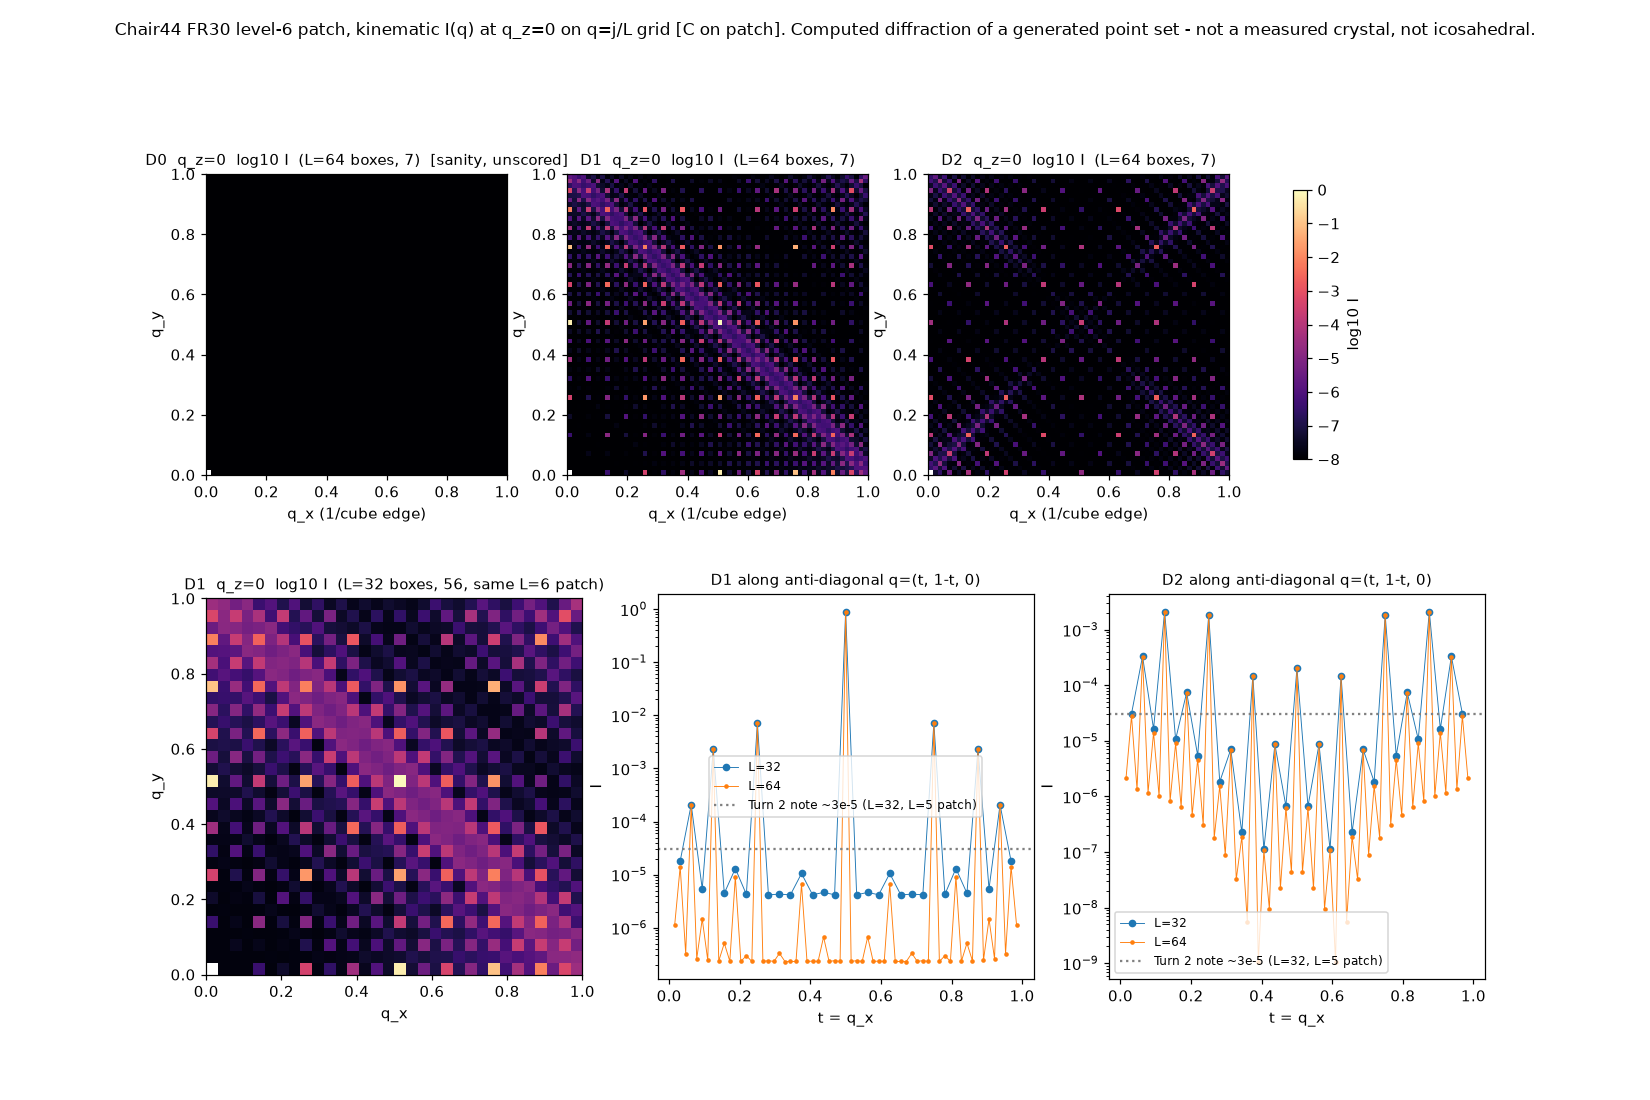
\includegraphics[width=\textwidth]{chair44_L64_qz0_streak.png}
\caption{Chair44 FR30 level-6 patch: kinematic intensity on the $q_z=0$ plane, $q=j/L$ (log scale), for decorations D0 (sanity), D1 and D2 [A] in boxes of side $L=64$, the D1 plane in $L=32$ boxes of the same patch, and the D1 and D2 intensities along the anti-diagonal $q=(t,1-t,0)$ at $L=32$ and $L=64$. Computed diffraction of a generated point set [C on patch]; not an observation, not a measured crystal, and not icosahedral. The fading D1 anti-diagonal is not a Bragg peak and not a diffuse sheet on this patch [X], and the figure makes no claim about the infinite hull; CH-V-020 stays [X]. Not a scored preregistered hypothesis. \textit{Provenance:} quasicrystal-materials/diffraction/figures/chair44\_L64\_qz0\_streak.png (sha256 \texttt{446f7757\ldots}), copied unchanged to figs\_v0.6/; data tables/chair44\_L64\_qz0\_streak.json; preregistration sha256 \texttt{10253440\ldots} (same patch).}\label{fig:streak}\end{figure}

\subsection{Three extensions used in Phase 3}
(1) Ensembles of connections from the Wilson measure $\exp(-\beta\sum_p(1-\tfrac12\mathrm{Re\,Tr}\,U_p))$ on the rigid-tile complex, $G\in\{Q_8,2I,SU(2)\}$ \cite{wilson1974confinement} (a standard pointer for the Wilson action; the action's normalisation and its use with the finite groups $Q_8$ and $2I$ are not checked from the abstract, and the journal body was not re-opened for this draft); (2) the $SU(2)$ deformation $U_\theta$ followed along $\theta=\kappa a$, $a=2^{-L}$; (3) a time direction, $T_L\times\mathbb{Z}_{N_t}$ with its transfer matrix (TOE\_ATTEMPT.md l.67--70).

\section{Results, gap by gap}\label{sec:results}
Each gap followed the same procedure: a frozen preregistration committed before any value it predicts was computed; implementation and run; scoring with the frozen rules, no refitting (TOE\_ATTEMPT.md l.74--79). The source was read from a file snapshot, not a git checkout, so the freeze order cannot yet be checked against commit history; Appendix~\ref{app:repro} lists the file hashes, seeds and run parameters that are known. \todo{prereg commit hashes and timestamps (G1, G2, G3, G5) and the toe repository commit: needed from the author}

\subsection{Gap 1: volume scaling of the matter floor}\label{sec:g1}
\textit{Model.} Independent Haar links ($\beta=0$) on pinned supertiles $T_1\ldots T_5$ (8 to 32\,768 tiles), groups $Q_8$, $2I$, $SU(2)$, 2780 samples (l.83--87).
\paragraph{Theorems used.}
\useclaim{G1-T1}\useclaim{G1-T2}\useclaim{G1-T3}\useclaim{G1-RARE}
\paragraph{Proof of T3 (from TOE\_ATTEMPT.md l.93; hand proof).} Let $G$ be finite and $n_p$ the number of plaquettes per link. Given everything outside a ball $B$, the conditional probability that all links of $B$ are trivial is at least $(e^{-2\beta n_p}/|G|)^{|B|}=:\delta_r>0$, uniformly in the outside configuration. Over infinitely many disjoint balls of radius $r$, successive conditioning gives $P(\text{no trivial ball among the first }n)\le(1-\delta_r)^n\to0$, so a trivial ball of radius $r$ exists almost surely, for every $r$. The Dirichlet ground state of a trivial ball of radius $r$ is a test vector for $H_U$ with Rayleigh quotient tending to $0$ as $r\to\infty$. Hence $\inf\sigma(H_U)=0$ almost surely. $\square$ This write-up is the author's and is not claimed new; it extends an earlier $\beta=0$ argument of the author to every $\beta$. Nakamura records $\inf\sigma=0$ almost surely in a different model (i.i.d.\ $U(1)$ fields on $\mathbb{Z}^2$) \cite{nakamura2000lifshitz}; that paper is not the source of the finite-energy and Borel--Cantelli argument above, and it does not treat Gibbs measures at $\beta>0$, non-abelian finite groups, or a substitution hull.
\paragraph{Results (simulated).}
\useclaim{G1-FLOORS}\useclaim{G1-TRIVIAL}\useclaim{TOE-G1-T1}\useclaim{TOE-G1-T2}
\paragraph{Scores (frozen rules).}
\useclaim{TOE-G1-H1}\useclaim{TOE-G1-H2}\useclaim{TOE-G1-H3a}\useclaim{TOE-G1-H3b}\useclaim{TOE-G1-H4}
\paragraph{Reading.} A descriptive, non-preregistered geometric extrapolation of the decrements (2.49, 0.99, 0.42, 0.25) would suggest an infinite-volume gap near 14; T3 shows this is false, and the plateau is pre-asymptotic (l.113--115). The extrapolation is not a claim of this note and is not labelled.
\useclaim{SC-8}

\subsection{Gap 2: a scaling region and a continuum limit}\label{sec:g2}
\subsubsection*{Part B: the $\theta$-trajectory of the frame connection}
\textit{Model.} $U_\theta$, rules FR30 and 1387, levels $T_1\ldots T_6$ (up to 262\,144 tiles); along $\theta_L=\pi2^{-L}$ the gauge part of the floor in physical units is $G_L=4^L(\lambda(\theta_L)-\lambda_1)\to\pi^2c_\infty$ provided $c_L$ converges (l.126--130).
\useclaim{G2B-DERIV}
(G2B-DERIV is the Phase~3 form of the expansion; its proved form is Theorem~A below, \texttt{TOE-PROOF-A}.)
\useclaim{G2B-CL}
All $c_L$ are deterministic floating-point solves, so they carry no statistical error bars: the resolvent equations are solved by conjugate gradients with relative tolerance $10^{-12}$ (src/pert.py), and the recorded maximum relative residual is about $10^{-12}$ or below (results/g2\_partB.json). The B2 extrapolation formula $c_\infty=c_6+(c_6-c_5)r/(1-r)$, $r=(c_6-c_5)/(c_5-c_4)$, was fixed in the preregistration (prereg/G2\_scaling.json); its sensitivity to the fitting range is given in the claim.
\useclaim{TOE-G2-B0}\useclaim{TOE-G2-B1}\useclaim{TOE-G2-B2}\useclaim{TOE-G2-B3}\useclaim{TOE-G2-B4}
\useclaim{G2B-LIMIT}\useclaim{G2B-MASS}\useclaim{G2B-POSTHOC}
\paragraph{Reading [X].} For the linearised $\theta$-family only, and if the conjectures G2B-LIMIT and G2B-MASS hold, no non-Abelian field survives the limit: the rapidly oscillating frame field homogenises and only a mass term remains (TOE\_ATTEMPT.md l.156--157). This reading is a conjecture; it is unlabelled in the source and printed here as [X]. An alternative reading is not excluded by the data: the six levels may still be pre-asymptotic (the B1 ratios fall from $0.53$ to $0.38$ for FR30), and the second-order coefficient says nothing about higher orders in $\theta$, where interacting terms could survive.

\subsubsection*{Proved afterwards: the $\theta\to0$ limit (PROOF.md)}
PROOF.md states that its proof ``is written and checked here; it is not machine-checked and not peer-reviewed'' (PROOF.md \S0 item 4); all its [P] items therefore carry \unverifiedtag.
\useclaim{TOE-PROOF-A}\useclaim{TOE-PROOF-B}\useclaim{TOE-PROOF-C}\useclaim{TOE-PROOF-D}
\useclaim{TOE-PROOF-E-FR30}\useclaim{TOE-PROOF-E-1387}\useclaim{PROOF-E-TABLE}
\useclaim{TOE-PROOF-prim}\useclaim{TOE-PROOF-F}\useclaim{PROOF-L7}
\paragraph{How the certified numbers depend on the hand proofs.} The numbers $\mu_\ell$ and $\nu^0_\ell$ are certified computations [C]. The certificate is a floating-point computation with explicitly bounded rounding error (PROOF.md \S5 ``Rounding'' and Lemma~6), not interval arithmetic, so the [C] status itself rests on two further hand-proved estimates. That the numbers bracket $\liminf c_L$ and $\limsup c_L$ uses Theorems~B and C; that they bracket $\rho(d)=\lim c_L$ uses Theorem~F. All three are hand proofs [P, unverified]. The brackets are therefore conditional statements.
\paragraph{Scope of the cited theorems.} PROOF.md \S6.1 cites Solomyak \cite{solomyak1997dynamics,solomyak1999corrections} for unique ergodicity, identifies the substitution matrix with the frame-walk matrix, and passes from $\mathbb{R}^3$ to $\mathbb{Z}^3$ through the suspension. Both steps are stated briefly in the source. Unique ergodicity of this framed-chair hull remains an unverified input. Solomyak's 1999 correction removes the implication from matrix primitivity to repetitivity; the original 1997 theorem's full hypotheses have not been checked from its body here. The later Lee--Moody--Solomyak paper \cite{lee2003consequences}, Theorem~4.1, proves unique ergodicity for FLC fixed points of primitive geometric tile substitutions without a separate repetitivity assumption, but the identification of our frame walk with such a substitution and the passage to the discrete $\mathbb{Z}^3$ suspension base remain unchecked. This [S] step is not treated as newly checked [P], and citing \cite{lee2003consequences} does not check it. A novelty-note scope check (theorem-F-novelty.md \S5.3) finds both the substitution-matrix identification and the $\mathbb{R}^3\to\mathbb{Z}^3$ suspension step plausible but stated only briefly in the source; a later scope check (solomyak-S-scope-check-2026-11-07.md) could not obtain the 1997 or 1999 paper bodies. Wiener's paper \cite{wiener1939ergodic} is cited in PROOF.md for the multiparameter pointwise ergodic theorem with cube averages; Wiener states his theorem for averages over balls of a continuous $\mathbb{R}^n$-action, while Lemma~7 uses cubes $Q_R$ in $\mathbb{Z}^3$. This cube-versus-ball mismatch is a documented gap, not a newly verified ergodic input. Suggested cube-average theorems (N.~Dunford, Acta Sci.\ Math.\ Szeged 14 (1951) 1; A.~Zygmund, Fund.\ Math.\ 38 (1951) 1) are not in the verified bibliography and are not cited here.

\paragraph{A provisional seventh level.} A level-$\ell=7$ certificate run has been queued and run but its results are not committed to the source (compute-queue/queue.jsonl, job \texttt{toe-l7-cert}; result files on the author's machine). Its notes give $\mu_7\ge13.291755$, $\tilde\nu_7\le14.480830$ (FR30) and $\mu_7\ge14.219208$, $\tilde\nu_7\le15.407377$ (1387), with $\tilde\nu_7=\nu^0_7+48\cdot2^{-7}$. Whether these values were rounded outward has not been checked; padding each end by $10^{-6}$ gives $[13.291754,14.480831]$ and $[14.219207,15.407378]$, both inside the $\ell=6$ brackets and both containing $c_6$ and the extrapolated $c_\infty$. Label: [C] \pendingtag{PROVISIONAL: uncommitted run, rounding direction unverified}. These numbers are not used anywhere else in this note; the headline brackets remain the $\ell=6$ ones.

\begin{table}[h]\centering\small
\caption{Certified level densities [C], rounded outward to six decimals from the stored full-precision bounds (toe/results/proof\_bounds.json, sha256 \texttt{b6752b18\ldots}): lower bounds rounded down, upper bounds rounded up. Ten cells differ from the values printed in PROOF.md \S5 (l.173--182); they are marked $^{a}$ and the printed value is given below.}\label{tab:munu}
\begin{tabular}{ccccc}\toprule
$\ell$ & $\mu_\ell\ge$ (FR30) & $\nu^0_\ell\le$ (FR30) & $\mu_\ell\ge$ (1387) & $\nu^0_\ell\le$ (1387)\\\midrule
1 & 6.780961$^{a}$ & 16.500001$^{a}$ & 7.197628 & 17.250001$^{a}$\\
2 & 10.596162 & 21.194785 & 11.401115 & 22.158938$^{a}$\\
3 & 12.203877$^{a}$ & 20.507430 & 13.276907$^{a}$ & 21.414960\\
4 & 12.841639 & 17.829293 & 13.812599$^{a}$ & 18.735685\\
5 & 13.109415 & 15.858983$^{a}$ & 14.046759$^{a}$ & 16.779928\\
6 & 13.232574 & 14.715589 & 14.161980 & 15.640966$^{a}$\\\bottomrule
\end{tabular}
\par\smallskip\footnotesize\raggedright $^{a}$\,Value printed in PROOF.md: FR30 $\mu_1=6.780962$, $\nu^0_1=16.500000$, $\mu_3=12.203878$, $\nu^0_5=15.858982$; 1387 $\nu^0_1=17.250000$, $\nu^0_2=22.158937$, $\mu_3=13.276908$, $\mu_4=13.812600$, $\mu_5=14.046760$, $\nu^0_6=15.640965$. PROOF.md says ``All values are rounded outward'', but these ten were rounded to nearest and lie on the unsafe side of the stored bounds by at most $5\cdot10^{-7}$ (discrepancies.md \S1). The source file is unchanged; correcting it is the author's decision.
\par\smallskip $^{b}$\,Headline brackets: FR30 $[13.232574,\,15.465590]$, 1387 $[14.161980,\,16.390966]$ (PROOF.md l.184--185). Both are on the safe side. For FR30 the stored upper end is $\nu^0_6+48/64=15.465588903524477$; its tight outward value is $15.465589$, which the ledger prints, and PROOF.md prints the valid but looser $15.465590$. This note keeps $15.465590$.
\end{table}

\paragraph{Not proved in PROOF.md.} The scaling trajectory (B3 stays [E]); the 13\,130 imprimitive rules (including x539311, x539291), for which only D holds; the uniform spectral shift B4; machine checking or independent review (PROOF.md \S0 l.21--25).

\subsubsection*{Part A: $Q_8\to2I\to SU(2)$ Wilson ensembles}
\textit{Model.} Rigid-tile complex on $T_2$ (576 links) and $T_3$ (5376 links); $\beta\in\{0.5,\ldots,64\}$; two chains, 500 thermalisation sweeps and 200 measurements per point (l.169--172). D2 (an angular-resolution estimate, unlabelled in the source and not used as support) gives $\beta_\times(2I)=12.4$, $\beta_\times(Q_8)=2.0$ (l.178). \todo{label for D2: needs the author; it is an estimate, so no stronger than [X]}
\useclaim{TOE-G2-D1}
\begin{table}[h]\centering\small
\caption{G2 Part A [E]: $R=\beta(\langle\lambda\rangle-\lambda_1)/C_{\rm pert}$ with one standard error, from toe/results/g2\_score.json (Part A table). $C_{\rm pert}=11.4856$ ($T_2$), $13.6306$ ($T_3$). Per point: two chains, 500 thermalisation sweeps, 200 measurements every 5 sweeps; the hot chain is scored at $\beta\le2$, the cold chain at $\beta\ge4$. Seed 20261031 (prereg/G2\_scaling.json).}\label{tab:R}
\begin{tabular}{crrrr}\toprule
$\beta$ & $SU(2)$, $T_2$ & $SU(2)$, $T_3$ & $2I$, $T_3$ & $Q_8$, $T_3$\\\midrule
0.5 & $0.4498(8)$ & $0.4505(5)$ & $0.4504(4)$ & $0.4472(5)$\\
1 & $0.8010(21)$ & $0.8067(9)$ & $0.8072(10)$ & $0.7775(11)$\\
2 & $1.1614(38)$ & $1.1961(19)$ & $1.1993(19)$ & $0.0215(4)$\\
4 & $1.1388(54)$ & $1.1825(24)$ & $1.1786(25)$ & $0.0000$\\
8 & $1.0633(58)$ & $1.0813(24)$ & $0.8753(26)$ & $0.0000$\\
16 & $1.0331(47)$ & $1.0381(23)$ & $0.0010(1)$ & $0.0000$\\
32 & $1.0249(42)$ & $1.0167(21)$ & $0.0000$ & $0.0000$\\
64 & $1.0017(43)$ & $1.0103(21)$ & $0.0000$ & $0.0000$\\\bottomrule
\end{tabular}
\par\smallskip\footnotesize\raggedright Entries $0.0000$: frozen ensemble, floor equal to $\lambda_1$ to four decimals (standard error below $10^{-4}$).
\end{table}
\useclaim{TOE-G2-W1}\useclaim{TOE-G2-W2}\useclaim{TOE-G2-W3a}\useclaim{TOE-G2-W3b}\useclaim{TOE-G2-W3c}\useclaim{TOE-G2-W4}
\useclaim{G2A-SELFENERGY}
\paragraph{Reading.} $2I$ has a narrow perturbative window ($\beta\approx2$--$8$) and then freezes between $\beta=8$ and 16, bracketing the estimate $12.4$; $Q_8$ deviates earlier than estimated (W3c [F]) (l.206--208). Table~\ref{tab:R} shows the pattern: $SU(2)$ approaches $R=1$ from above for $\beta\ge4$; $2I$ follows $SU(2)$ up to $\beta=4$, drops to $0.875$ at $\beta=8$ and is frozen from $\beta=16$; $Q_8$ already departs at $\beta=1$ ($0.7775\pm0.0011$ against $0.8067\pm0.0009$) and is frozen from $\beta=2$. In raw floors the $\beta\le1$ departure of $Q_8$ is $13.862\pm0.014$ against $13.950\pm0.014$ at $\beta=0.5$, and $12.267\pm0.016$ against $12.666\pm0.013$ at $\beta=1$ ($T_3$).

\subsection{Gap 3: a time direction}\label{sec:g3}
\textit{Model.} Wilson theory on $T_2\times\mathbb{Z}_8$ with rigid tiles, $\beta\in\{0.25,0.5,1\}$, 20\,000 heat-bath measurements per run \cite{kennedy1985heatbath} (l.212--215). Two-link plaquettes (483 per slice on $T_2$) give $r(1)=u_G(\beta)^2$ at leading order and $m=-2\ln u_G$ (l.222--225).
\useclaim{TOE-G3-R0}
Lüscher constructs a self-adjoint, strictly positive, gauge-invariant transfer matrix for $SU(N)$ on a four-dimensional hypercubic lattice \cite{luscher1977transfer}; that mechanism does not cover $Q_8$, $2I$, or an arbitrary spatial 2-complex. Osterwalder--Seiler is cited as a standard pointer for a positive self-adjoint transfer matrix \cite{osterwalder1978gauge} (abstract only; the proof, gauge choice, and group class were not seen). R0's extension to the present setting remains [P, unverified].
\useclaim{TOE-G3-R1}\useclaim{TOE-G3-R2}\useclaim{TOE-G3-R3a}\useclaim{TOE-G3-R3b}\useclaim{TOE-G3-R3c}
\useclaim{G3-SPECTRUM}\useclaim{SC-6}
\paragraph{Uncertainties for G3.} Each G3 run has 20\,000 measurements (results/g3\_score.json). One standard error of $r(1)/u^2$, computed as $\sigma_{r(1)}/u^2$ from that file: $\beta=0.25$: $0.027$, $0.033$, $0.030$; $\beta=0.5$: $0.011$, $0.010$, $0.010$ (for $2I$, $Q_8$, $SU(2)$). The file records no error for $m_{\rm eff}$, so R3c is scored without one.
\paragraph{Reading.} This is not Lorentzian 3+1 physics: space and time are treated differently, and $Q_8$ has no continuum limit (l.240).

\subsection{Gap 4: chirality (obstruction recorded)}\label{sec:g4}
No preregistration was frozen because no computation was run (l.245).
\useclaim{TOE-G4-O1}\useclaim{TOE-G4-O2}\useclaim{G4-INFVOL}
Nielsen--Ninomiya are cited as pointers for the 1981 no-go theorem \cite{nielsen1981absenceI,nielsen1981absenceII} (abstracts only). The draft's ``finite-volume content'' reading cannot be checked from those abstracts; the infinite-volume, translation-invariant proofs do not cover the finite-patch claim as stated (G4-INFVOL). A domain wall inserts chirality rather than deriving it \cite{kaplan1992chiral}; no verified citation for an overlap operator is inserted here. An $SU(2)$ theory with an odd number of left-handed doublets (and no other representations) is inconsistent \cite{witten1982su2} (abstract pointer; statement pages were not seen).

\subsection{Gap 5: generations}\label{sec:g5}
The only threefold structure is the set of three $\mathbb{Z}_2$ shadows $\chi_1,\chi_2,\chi_3$, the non-trivial characters of $V_4=Q_8/\{\pm1\}$ (l.264).
\useclaim{G5-S1}\useclaim{TOE-G5-S3}\useclaim{G5-S4}\useclaim{G5-COUNT}
\useclaim{TOE-G5.1}\useclaim{TOE-G5.2}\useclaim{TOE-G5.3}\useclaim{TOE-G5.4}\useclaim{TOE-G5.5}
\useclaim{TOE-G5-none}\useclaim{G5-R63}

\subsection{Gap 6: gravity (obstruction recorded)}\label{sec:g6}
The two claims below are separate from the T1 gravity run. Where this note mentions that run: the $L=1$ interior count is $0$, not $6$; $N_{\mathrm{int}}=6$ holds at $L=2,\ldots,5$ [C]; no local tile-wise moduli, and $Q=0$, are [C] only at $L=1,\ldots,5$ in this tile-wise constant, tangentially continuous metric model; the all-level claim is [X]. This is not a classification of all Regge formulations.
TOE-G6-O1 is an elementary geometry statement that Regge deficits vanish on the chair complex (a hand proof, unverified); it is not T1's ``no local moduli'' result, and ``rigid'' in the claim text should not be read that way. ``Regge calculus'' is used here as a name \cite{regge1961coordinates} (pointer only; the deficit-angle definition and the action were not seen from the abstract), not as support for the chair-complex deficit-zero calculation.
TOE-G6-O2 (that dynamical geometry leaves the substitution class) is a one-line remark in TOE\_ATTEMPT.md \S3.6, also unverified. Causal dynamical triangulations are a standard way to make the geometry dynamical \cite{ambjorn2004emergence}; that reference does not support the claim that doing so leaves the substitution class or destroys legal-patch structure.
\useclaim{TOE-G6-O1}\useclaim{TOE-G6-O2}

\section{Scorecard after Phase 3}\label{sec:scorecard}
\begin{table}[h]\centering\small
\caption{Scorecard (TOE\_ATTEMPT.md \S4 l.310--321, identical to SCORECARD.md). Partial-result labels in rows 3 and 4 are restated with the paper labels of Appendix~\ref{app:labelchanges}; the source prints ``[P]/[C]'' for row 3 and ``one continuum trajectory [E]'' for row 4. The [P] entries are hand proofs [P, unverified].}
\begin{tabular}{@{}cp{0.38\textwidth}p{0.22\textwidth}p{0.25\textwidth}@{}}\toprule
\# & requirement & status & partial results\\\midrule
1 & $SU(3)\times SU(2)\times U(1)$ & missing & $SU(2)$ as dynamical field [E]\\
2 & chiral fermions & missing & obstruction (G4)\\
3 & three generations & missing & obstruction (G5): [P] S3; [C] symmetry count; [E] floor equalities\\
4 & Lorentzian 3+1 and continuum limit & missing & lattice time direction [P]; one $\theta$-trajectory, $L\le6$ [E]; its continuum limit [X]\\
5 & general relativity in some limit & missing & obstruction [P] (G6)\\
6 & QM with unitary time evolution & \claimtag{P} lattice level only & G3 R0 (standard)\\
7 & dimensionless constants, derived & missing & model constants derived [E]\\
8 & (internal) floor as order parameter & \claimtag{P} negative & G1 T3\\\bottomrule
\end{tabular}
\end{table}
Rows open: 1, 2, 3, 4, 5, 7.\footnote{The source README.md says ``One scorecard row is [P]''; SCORECARD.md has row 6 [P] and row 8 [P] negative (discrepancies.md \S2.7). Row 8 is programme-internal, not a physics requirement.}

\section{What would falsify this}\label{sec:falsify}
Each label comes with its own refutation route (TOE\_ATTEMPT.md \S5 l.324--339).
\begin{itemize}
\item \textbf{[P] claims} (hand proofs: the diamagnetic bound and compression T1, T2, the infinite-volume statement T3, the transfer-matrix positivity R0, the obstructions of G4--G6, Theorems A--F) are refuted by a counterexample or by an error in the argument. A finite-group Wilson ensemble with a positive infinite-volume floor at some $\beta$ would refute T3; a primitive frame rule for which $c_L$ does not converge would refute Theorem~F.
\item \textbf{[C] claims} are refuted by an independent recomputation that disagrees, or by an error in the rounding analysis on which the certificates rest. A value of $c_L$ for FR30 or 1387 at some large $L$ outside the certified bracket (beyond the finite-$L$ factor of Theorem~C) would refute the bracket or one of Theorems B, C, F.
\item \textbf{Preregistered [E] predictions} are refuted by reruns outside the frozen bands: new seeds, larger levels, more chains, or an independent implementation. The frozen protocols and seeds are listed in Appendix~\ref{app:repro}.
\item \textbf{[X] claims}: the continuum-limit conjectures G2B-LIMIT and G2B-MASS would be refuted by levels $L\ge7$ whose $c_L$ leave the certified bracket or stop converging geometrically, or by a non-vanishing higher-order term that survives $\theta=\kappa a\to0$.
\end{itemize}
The programme as a route to interacting physics is already close to refuted. If the $\theta$-trajectory limit is free for every rule and every $\kappa$, the core carries no interacting continuum physics. That general statement is open; it has been checked only for FR30 and 1387 and only at second order in $\theta$.

\section{Novelty and relation to prior work}\label{sec:novelty}
No result here is claimed new except the elementary G5 statement about Chair44 rules (G5-COUNT [C]) and the specific application of homogenisation described in \S\ref{sec:relwork} (TOE\_ATTEMPT.md \S6 l.341--355).
\begin{itemize}\small
\item G1 T3: the finite-energy and Borel--Cantelli write-up is the author's and is not claimed new. Nakamura records $\inf\sigma=0$ almost surely in a different model \cite{nakamura2000lifshitz} and is not cited as the source of that argument.
\item G1 H1/H2: generic pointer for Poisson statistics \cite{minami1996local} (Minami treats bulk local statistics of the i.i.d.\ Anderson model, not ground-state or extreme-value laws for random $Q_8$ connections on nested supertiles; those claims are already [F]). No novelty is claimed.
\item $2I$ freezing: first-order / freezing behaviour for $2I$ is recorded in \cite{petcher1980montecarlo} (abstract only). That paper is not cited for $Q_8$ or for the spherical-design argument, which were not seen in the abstract.
\item G2 Part A self-energy: standard mechanism, no new method. No verified weak-coupling reference for the $C/\beta$ self-energy is in the bibliography, and none is inserted here.
\item G3 R0, G4, G6: standard (citations as in \S\ref{sec:g3}, \S\ref{sec:g4}, \S\ref{sec:g6}).
\end{itemize}

\subsection{Related work: homogenisation and Theorem F}\label{sec:relwork}
Theorem~F is an application of known ergodic (stochastic) homogenisation results to the framed-chair hull; it is not a new limit theorem. A novelty check of Theorem~F (research-publishing/novelty/theorem-F-novelty.md, 2026-10-31, status PARTIAL: the search stopped early under a rate limit, and Semantic Scholar and Google Scholar were not queried) reaches the following conclusions, which this section adopts.
\begin{itemize}\small
\item \textbf{The corrector formula is standard.} $\rho(d)=7\min_{\xi\in\mathcal C}E_\mu\sum_k|w_k+\xi_k|^2$, with minimiser $-P_{\mathcal C}w$, is the discrete corrector (homogenised-coefficient) formula of Kozlov \cite{kozlov1987difference} and of K\"unnemann \cite{kunnemann1983diffusion} (not written there in $\min$ / $-P_{\mathcal C}w$ form). The continuum variational form is Kozlov's 1979/80 averaging paper \cite{kozlov1980averaging}; the discrete formula is the 1986/87 difference-scheme paper. A continuum formula of Papanicolaou and Varadhan was cited in an earlier draft; that paper is not in the verified bibliography and is not cited here.
\item \textbf{Convergence of periodised approximations is known in ergodic media.} Convergence of periodised effective coefficients to the homogenised one is proved by Owhadi \cite{owhadi2003periodization}. Convergence of more general finite-box approximations was previously attributed to Bourgeat and Piatnitski; that paper is not in the verified bibliography and is not cited here.
\item \textbf{Homogenisation on aperiodic tilings is known.} Braides, Riey and Solci homogenise energies on Penrose tilings \cite{braides2009penrose}. Telcs proves an invariance principle on the Penrose tiling by an environment-process method \cite{telcs2010penrose}; the corrector method on that tiling is Bartha and Telcs \cite{bartha2013penrose}.
\item \textbf{Deterministic and survey references.} Biskup's survey of the random conductance model \cite{biskup2011survey} is the standard reference for the discrete corrector, and his work on deterministic conductances \cite{biskup2025deterministic} treats homogenisation without randomness.
\item \textbf{The $\theta^2$ link.} That the second-order coefficient of the lowest eigenvalue of the twisted operator equals a homogenised coefficient (Theorems~A and F together) is analogous to Bloch-wave homogenisation [A] \cite{conca1997bloch} (metadata verified; content not checked).
\end{itemize}
What is specific to this note, and possibly new only in combination (novelty note \S3, verdict ``partially anticipated''): (i) the finite-volume problems are Perron-weighted problems on pinned supertiles $T_L$ with free boundary, rather than periodised or Dirichlet boxes; (ii) the limit is deterministic along the single sequence $T_L$, the ergodic input being unique ergodicity of the substitution hull \cite{solomyak1997dynamics,solomyak1999corrections} rather than an average over a random environment (unique ergodicity of this hull remains an unverified input; see the scope remarks in \S\ref{sec:g2}); (iii) the $\theta^2$ link above. No rate of convergence is proved; a quantitative rate for $|c_L-\rho|$ would go beyond the cited literature and would tighten the certified brackets.
Theorem~F also uses a multiparameter ergodic theorem \cite{wiener1939ergodic} and Kolmogorov--Riesz compactness \cite{hancheolsen2010kolmogorov}; the Wiener citation is a documented cube-versus-ball gap, not a newly verified input (see \S\ref{sec:g2}).
Dorodnyi (arXiv:2005.06516, 2020) treats periodic homogenisation, including periodic magnetic examples; it does not cover the substitution hull, so it does not apply to G2 Part B or Theorem F.

\section{Where it stands}\label{sec:stands}
The certified mathematics of the core stands: the results K1--K15 and the certified numbers of Corollaries D and E do not depend on any physics reading. What Phase~3 adds is a set of lattice-level facts and one conditional limit statement.
\begin{itemize}
\item For finite gauge groups the matter floor is not an infinite-volume order parameter (T3, SC-8).
\item In the dynamical $SU(2)$ theory the gauge-induced floor shift is the perturbative self-energy, to 1\,\% at $\beta=64$ (G2A-SELFENERGY [E]); $2I$ and $Q_8$ freeze as designed, $Q_8$ earlier than predicted (W3c [F]).
\item Adding a time direction gives a positive transfer matrix and the derived strong-coupling spectrum (R0, G3-SPECTRUM), but not Lorentzian 3+1 physics.
\item Along the $\theta$-trajectory the second-order coefficient converges (Theorem F, for primitive rules) and is certified to lie in an interval of width about $2.23$ for FR30 and 1387 (Corollary E, conditional on Theorems B, C, F); numerically it behaves like a mass term for $L\le6$ [E], and the continuum limit is a conjecture [X].
\end{itemize}
Every limit found so far looks like free physics, and the substitution hull acts as an inert lattice (TOE\_ATTEMPT.md l.390). Chirality, generations and gravity carry recorded obstructions, not partial successes.

\section{Phase summaries}\label{sec:phases}
Phase~0 labelled 1243 claims from the work. Of these, 327 are excluded (the excluded lineage, together with every claim already marked [F]); 139 rest on hard-coded tests; and 192 Lean theorems whose names promised more than they proved were relabelled. All eight Chair44 certificate files were re-checked by the Lean~4.35.0 kernel and use only standard axioms. Phase~0 itself recorded no new failure; the audit confirms earlier refutations already marked [F].

Phase~1 stated the core object in CORE.md and listed the proved and certified properties K1--K15. What fits is the Chair44 work, the Tseitin $\mathbb{Z}_2$ coboundary results, and the Unique Games reading; what does not fit is random 3-SAT, solver and ML engineering, and the 6D$\to$3D icosahedral modules. The Unique Games reading (K11) is the source's recommended bridge between the complexity work and the floor.

Phase~2 recorded a baseline in which every physics scorecard row was missing, with seven no-go facts each traced to a source. The recommended first attacks were the volume question and the continuum question.

Phase~3 ran the preregistered gap attacks. Row~6 became [P] at the lattice level (G3). Row~4 gained a lattice time direction [P] and one $\theta$-trajectory at finite $L$ [E]; identifying that trajectory's limit as a continuum or mass term remains [X] in this note (owner ledger sync, 6~November 2026). Row~8 was settled negatively [P]. Rows~2, 3 and~5 now carry explicit obstructions: for row~3 the obstruction itself is [P] (S1/S4), the symmetry count is [C], and the numerical degeneracies (G5.1--G5.4) are [E]. The Phase~3 failures, all recorded as [F], were G1~H1 (weakest-child localisation), G1~H2 (min-stable law at $L=3,4$), G1~H3b ($Q_8$ significantly below $SU(2)$), G2~W3c ($Q_8$ tracks $SU(2)$ at $\beta\le 1$), and G2~B4 (a uniform shift of 20 levels at $L=5$; a post-hoc diagnostic points to an eigensolver artifact). Other preregistered items were not falsified in Phase~3. The recommended next step was to prove the G2 Part~B homogenisation limit.

After Phase~4 that step was written in PROOF.md. No scorecard row moved, because the limit is free physics. What moved from [E] to a written proof [P, unverified] is the existence of $\lim c_L$ for primitive rules ($1\,666\,486$ rules), its identification as a hull corrector formula, and the uniform lower bound $3527/1012$ for all $6^8$ rules, together with certified brackets [C] for FR30 and 1387. Identifying those finite-level constants as a continuum mass term remains [X]. Still open are the $\theta^3$ remainder along the trajectory (B3 stays [E]); the $13\,130$ imprimitive rules, including x539311 and x539291, whose hull has two components and whose even- and odd-level convergence is open; and machine checking or independent review of the written proof. The source notes that a sloped or periodic cell problem would be a cheap way to tighten the upper end of the bracket, whose width is about $2.23$ at $\ell=6$.

\section{Figures}\label{sec:figures}
Figures 1--4 are identical to the frozen v1.0 set (no $\ell=7$ series), built from printed PROOF.md values or stored result files. Figure 5 was rebuilt for this draft from the outward enclosure $[7.954291,\,8.7642270382]$ [E]. The set lives in \texttt{figs\_v0.2/}; regenerate Figure 5 with \texttt{make\_figures.py --paper} (venv: matplotlib 3.11.2, numpy 2.5.4) after copying Figures 1--4 from \texttt{figs\_v1.0/}. Figures 1--4 plot the values \emph{as printed in PROOF.md}, including the ten nearest-rounded cells of Table~\ref{tab:munu}, which they flag. Labels inside the figure legends follow the source; where they differ from the paper labels, the caption gives the paper label, which applies.

\begin{figure}[h]\centering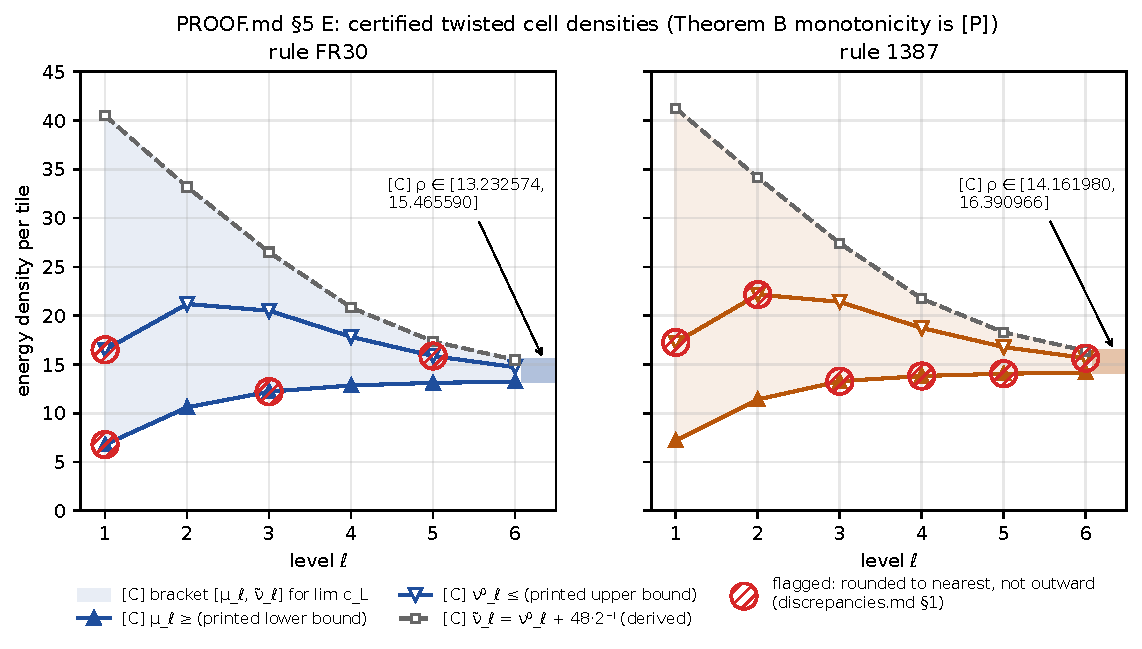
\includegraphics[width=0.9\textwidth]{fig1_mu_nu_vs_level.pdf}
\caption{Certified twisted cell densities for FR30 (left) and 1387 (right), $\ell=1$--6 (PROOF.md \S5 E, l.173--182). Filled triangles: $\mu_\ell\ge$ [C]; open triangles: $\nu^0_\ell\le$ [C]; grey squares: $\tilde\nu_\ell=\nu^0_\ell+48\cdot2^{-\ell}$ [C]. The shaded band $[\mu_\ell,\tilde\nu_\ell]$ encloses $\lim c_L$ conditional on Theorems B, C, F [P, hand proof, unverified]. Right-edge bar: certified bracket for $\rho(d)$ [C], conditional in the same way. Red hatched rings: the 10 cells printed in PROOF.md rounded to nearest rather than outward; the outward values are in Table~\ref{tab:munu} (differences $\le5\cdot10^{-7}$, invisible at this scale).
\textit{Provenance:} figures/proof-brackets/figs\_v0.2/fig1\_mu\_nu\_vs\_level.pdf (identical to frozen figs\_v1.0); data/brackets\_v1.0.json.}\end{figure}

\begin{figure}[h]\centering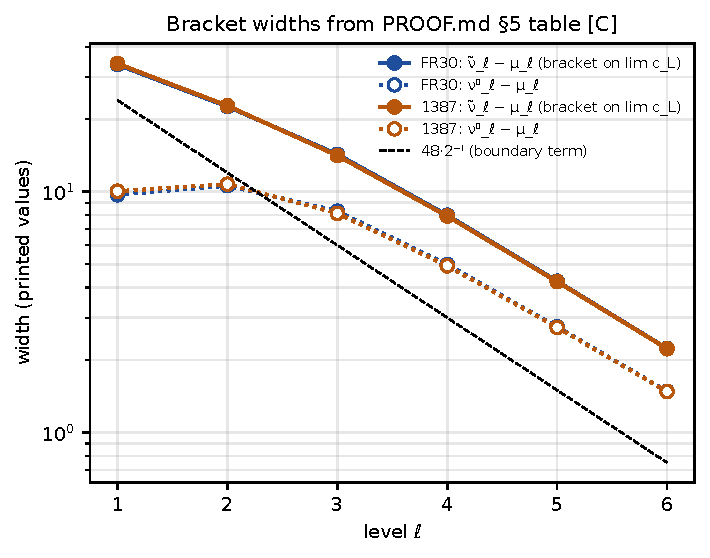
\includegraphics[width=0.75\textwidth]{fig2_bracket_widths.pdf}
\caption{Bracket widths (log scale) from the printed PROOF.md \S5 values [C]: $\tilde\nu_\ell-\mu_\ell$ (solid), $\nu^0_\ell-\mu_\ell$ (dotted), boundary term $48\cdot2^{-\ell}$ (dashed). At $\ell=6$ the width is $\approx2.23$ for both rules. No trend beyond $\ell=6$ is claimed. \textit{Provenance:} figs\_v0.2/fig2\_bracket\_widths.pdf (identical to frozen figs\_v1.0).}\end{figure}

\begin{figure}[h]\centering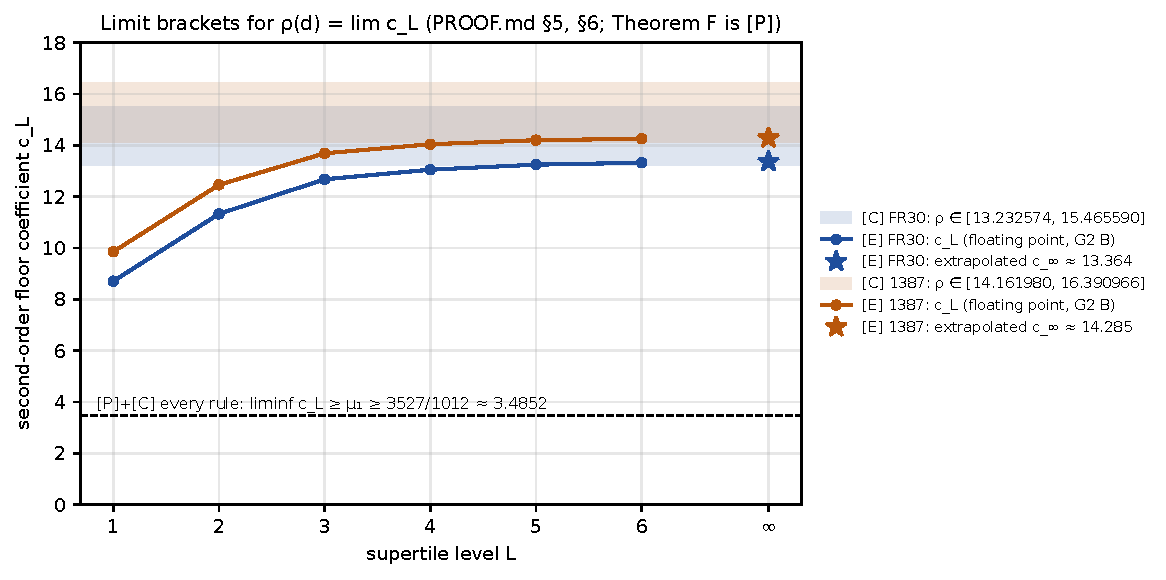
\includegraphics[width=0.75\textwidth]{fig3_limit_brackets.pdf}
\caption{Limit brackets for $\rho(d)=\lim c_L$: $\rho(\mathrm{FR30})\in[13.232574,15.465590]$, $\rho(1387)\in[14.161980,16.390966]$ [C], conditional on Theorems B, C, F [P, hand proof, unverified]. Dots: floating-point $c_L$, $L=1$--6, from G2 Part B [E]; they have no error bars because they are deterministic solves (conjugate gradients, relative tolerance $10^{-12}$, maximum relative residual about $10^{-12}$ or below). Stars: the preregistered B2 extrapolations $c_\infty\approx13.364$, $14.285$; an extrapolation beyond the data is printed here as [X] (the legend says [E]); changing the fitting range moves them by $0.10$ and $0.04$. Dashed: $\liminf c_L\ge3527/1012\approx3.4852$ [C] (the legend says [P]+[C]; the paper prints the weaker component). The legend's ``Theorem F is [P]'' means a hand proof, unverified. Finite-$L$ values are not bounded by the bands without the $\varepsilon_{\ell,L}$ factor of Theorem C. \textit{Provenance:} figs\_v0.2/fig3\_limit\_brackets.pdf (identical to frozen figs\_v1.0); results/g2\_partB.json.}\end{figure}

\begin{figure}[h]\centering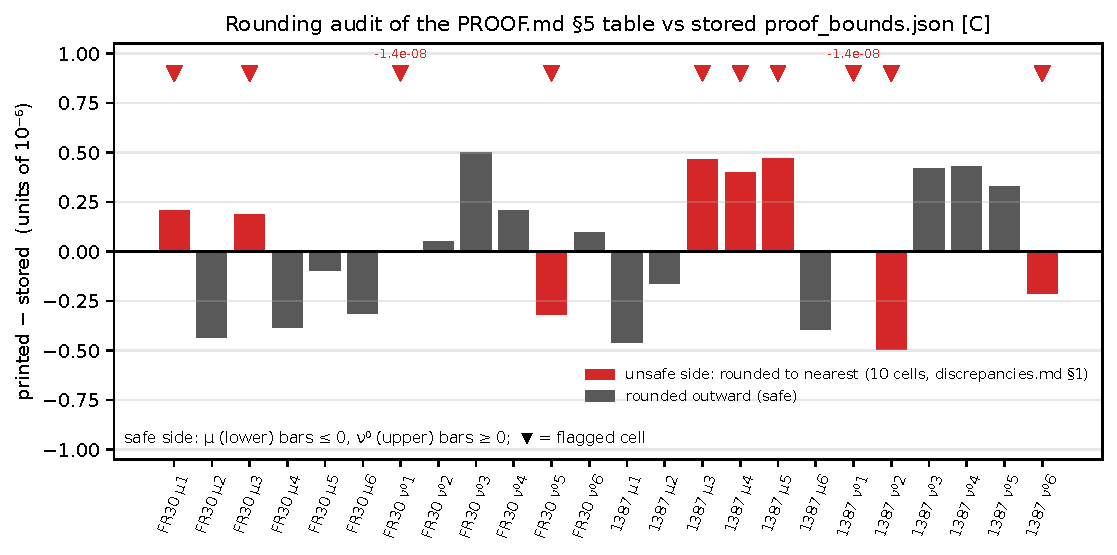
\includegraphics[width=0.75\textwidth]{fig4_rounding_audit.pdf}
\caption{Rounding audit: printed PROOF.md value minus stored unrounded certified bound (results/proof\_bounds.json), in units of $10^{-6}$, all 24 cells [C]. Red bars (\,$\blacktriangledown$\,) are the 10 cells on the unsafe side; they match discrepancies.md \S1. \textit{Provenance:} figs\_v0.2/fig4\_rounding\_audit.pdf (identical to frozen figs\_v1.0).}\end{figure}

\begin{figure}[h]\centering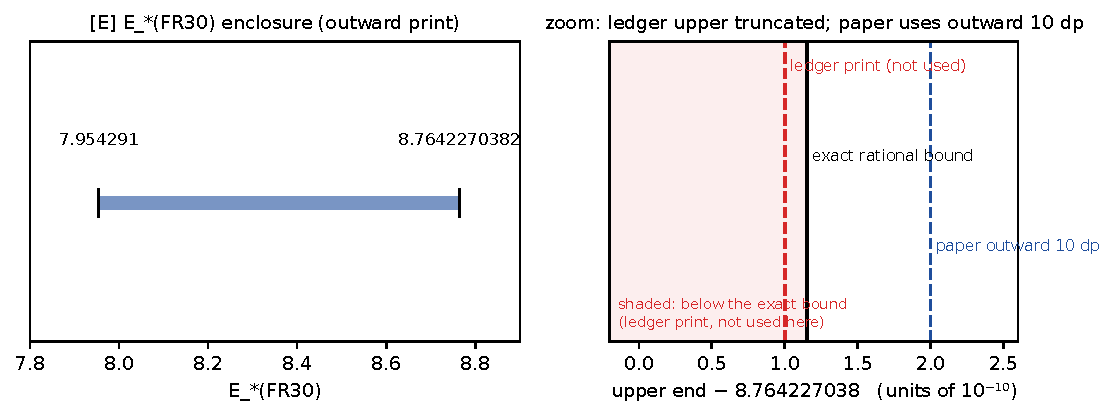
\includegraphics[width=0.85\textwidth]{fig5_Estar_FR30_enclosure.pdf}
\caption{The FR30 spectral-floor enclosure as printed in this note, rounded outward: $[7.954291,\,8.7642270382]$ [E], until ratification of the Phase~IX category-to-label mapping. The figure shows those outward values. The ledger prints $[7.954292,\,8.7642270381]$; that upper end is truncated and lies below the exact rational bound, so it is not a safe upper print (right panel).\protect\footnotemark\ \textit{Provenance:} figs\_v0.2/fig5\_Estar\_FR30\_enclosure.pdf; ledger.json l.474, l.624. Computed quantity, not observational.}\end{figure}
\footnotetext{Upper end: the exact certified bound is $95969095435322528/10950092349041091=8.764227038115\ldots$, so the outward 10-decimal value is $8.7642270382$ (discrepancies.md \S1). Lower end: there are two independent certificates, $7.954292265$ and $7.954291278$ (discrepancies.md \S2.3). The ledger's $7.954292$ is below the first but above the second, so it is not safe with respect to both; this note prints $7.954291$, which is below both. The paper label is [E] until ratification of the Phase~IX mapping that sent the source category to [C] (discrepancies.md \S2.2). The owner first pass of 6 November 2026 re-checked this outward arithmetic [C] and did not re-derive the certificates from source files. The source files are unchanged.}
\useclaim{FIG5-ESTAR}

\section{Limitations and open problems}\label{sec:limits}
\begin{itemize}
\item \textbf{Not a theory of everything.} Six of seven physics scorecard rows are open; the only [P] physics row (QM with unitary evolution) holds at lattice level and is a standard construction.
\item \textbf{Every limit found looks like free physics.} Along the $\theta$-trajectory, for $L\le6$, the second-order coefficient behaves like a mass term [E]; that a continuum limit exists and is a free massive field is a conjecture [X]. The $SU(2)$ regime of Part A is ordinary weak-coupling lattice gauge theory [E].
\item \textbf{Unverified proofs.} The PROOF.md argument (Theorems A--F, Lemmas 6 and 7, the rounding analysis) and the G1/G3/G4/G5/G6 [P] statements are hand proofs, not machine-checked and not peer-reviewed. The certified brackets and the bound $3527/1012$ depend on them. An external expert reading or a formalisation is needed before any of these loses its \unverifiedtag\ tag.
\item \textbf{Open mathematics.} Uniformity of the $\theta^3$ remainder along $\theta_L=\pi2^{-L}$ (B3 remains [E]); the 13\,130 imprimitive rules (even/odd-level limits); the infinite-volume chirality statement for the hull [X]; whether the $\theta$-trajectory limit is free for \emph{every} rule and $\kappa$.
\item \textbf{Falsified predictions.} G1 H1, H2, H3b; G2 W3c, B4; Phase XIV H1, H2; Phase VI gapped claim; QIS-299. B4's post-hoc diagnostic does not change its [F]; a new frozen protocol is needed.
\item \textbf{Finite sizes and statistics.} G1 up to $T_5$ only (the rare regions are estimated to appear near $10^{22}$ tiles, G1-RARE [X]); G2 A has two chains per point and 200 measurements, so autocorrelations are handled only through the 5-sweep spacing; G2 B has six levels, and its $c_\infty$ depends on the fitting range by up to $0.10$. Standard errors are given where the sources record them (G1 floors and H3, Table~\ref{tab:R}, G3 R3a); the G3 R2 standard errors are taken from results/g3\_score.json (Section~\ref{sec:g3}); the G3 R3c effective masses have no recorded error; seeds and run counts are in Appendix~\ref{app:repro}.
\item \textbf{Bounds hygiene.} Ten PROOF.md table cells are rounded to nearest, the ledger's $E_*$ upper end $8.7642270381$ is truncated, and its lower end $7.954292$ is above one of the two certificates; this note prints outward values (Table~\ref{tab:munu}, Appendix~\ref{app:labelchanges}). PROOF.md prints $15.465590$ and the ledger $15.465589$; both are safe. The source files are unchanged.
\item \textbf{Label mismatches with the ledger} (Appendices~\ref{app:flags} and \ref{app:labelchanges}): resolved here toward the weaker label. As of the 6 November 2026 owner ledger sync, the previously unmapped rows now use the paper id as the ledger id (recorded in claims.csv). Two paper labels, G1-RARE [X] and G2B-DERIV [E], still carry a pending author ruling on the source's non-standard P-level wording; no ruling is invented here. K6 keeps printing [C] as the weakest component of a compound whose X4 no-go remains [P] in the ledger.
\item \textbf{Reproducibility.} The source was read from a file snapshot; Appendix~\ref{app:repro} gives file hashes, seeds and parameters, but no commit hashes. \todo{toe repository commit and prereg commits: needed from the author}
\end{itemize}

\appendix
\section{Status of claims}\label{app:claims}
% generated
Total labelled claims: 99. By paper label: [P]~33, [C]~12, [E]~33, [X]~5, [A]~5, [F]~11. By source label (verbatim, including non-standard and compound labels): [A]~5, [C]~15, [E]~26, [E, post hoc]~1, [F]~11, [P]~34, [P+C]~2, [P-level]~1, [P-level estimate]~1, [P/C]~1, [X]~2. 15 claims carry a paper label different from their source label (Appendix~\ref{app:labelchanges}); 2 carry a pending-ruling marker. Of the claims printed [P], 32 are hand proofs marked \unverifiedtag.

% generated by build_claims.py -- do not edit by hand
\begin{longtable}{@{}>{\raggedright\arraybackslash}p{0.15\textwidth}>{\raggedright\arraybackslash}p{0.07\textwidth}>{\raggedright\arraybackslash}p{0.13\textwidth}>{\raggedright\arraybackslash}p{0.30\textwidth}>{\raggedright\arraybackslash}p{0.25\textwidth}@{}}
\toprule ID & Where & Label & Statement (short) & Evidence\\\midrule\endhead
\scriptsize\texttt{S1-QIS-PNP} & \scriptsize \S{}1 & \claimtag{F} & \scriptsize QIS 'unconditional P != NP' claim is refuted by the repo's own audit & \scriptsize TOE\_ATTEMPT.md \S{}8 l.401; CORE.md \S{}5 l.84; ledger.json QIS-322 [F, excluded as falsified]\\
\scriptsize\texttt{S1-QIS-PLANNER} & \scriptsize \S{}1 & \claimtag{F} & \scriptsize QIS '64-0 planner' record is refuted by the repo's own audit & \scriptsize TOE\_ATTEMPT.md \S{}8 l.401; CORE.md \S{}5 l.84; ledger.json QIS-182 [F, excluded as falsified]\\
\scriptsize\texttt{K1} & \scriptsize \S{}2.2 & \claimtag{P}\newline\unverifiedtag & \scriptsize flat \textless{}=\textgreater{} gauge-trivial \textless{}=\textgreater{} lambda\_min(H\_U)=0 on finite connected graphs & \scriptsize CORE.md \S{}2 l.38 (source: Chair44 X1)\\
\scriptsize\texttt{K2} & \scriptsize \S{}2.2 & \claimtag{P}\newline\unverifiedtag & \scriptsize E\_* = inf over legal patches of Dirichlet floor; depends only on legal environments & \scriptsize CORE.md \S{}2 l.39 (source: XII.A)\\
\scriptsize\texttt{K3} & \scriptsize \S{}2.2 & \claimtag{P}\newline\unverifiedtag & \scriptsize two-sided IMS localisation with optimal R\textasciicircum{}-2 rate & \scriptsize CORE.md \S{}2 l.40 (source: XII.B, XII.C)\\
\scriptsize\texttt{K4} & \scriptsize \S{}2.2 & \claimtag{P} & \scriptsize forced curvature: \textgreater{}=12 of 21 centre-octant two-cycles non-trivial (Lean checks encoded finite predicates only; geometric statement not kernel-checked) & \scriptsize CORE.md \S{}2 l.41 (source: Phase VII-B P1)\\
\scriptsize\texttt{K5} & \scriptsize \S{}2.2 & \claimtag{C} & \scriptsize all 1098 gauge classes of the 6561 proper rules have E\_* \textgreater{}= 3.788 & \scriptsize CORE.md \S{}2 l.42 (source: X3)\\
\scriptsize\texttt{K6} & \scriptsize \S{}2.2 & \claimtag{C}\newline\unverifiedtag\newline{\tiny source: P/C (App.~\ref{app:labelchanges})} & \scriptsize plaquette-class frequencies give no lower bound on E\_* & \scriptsize CORE.md \S{}2 l.43 (source: X4, X5, XII.P63); source label [P/C]\\
\scriptsize\texttt{K7} & \scriptsize \S{}2.2 & \claimtag{P}\newline\unverifiedtag & \scriptsize non-spinor floors are functions of the plaquette class field & \scriptsize CORE.md \S{}2 l.44 (source: XI.H3)\\
\scriptsize\texttt{K8} & \scriptsize \S{}2.2 & \claimtag{P}\newline\unverifiedtag & \scriptsize Orbit Lemma & \scriptsize CORE.md \S{}2 l.45 (source: XII.OL)\\
\scriptsize\texttt{K9} & \scriptsize \S{}2.2 & \claimtag{C} & \scriptsize certified E\_* enclosures for 1387 and 539311; maximiser among three rules & \scriptsize CORE.md \S{}2 l.46 (source: XII.R20, XII.r24, XII.F4)\\
\scriptsize\texttt{K10} & \scriptsize \S{}2.2 & \claimtag{C}\newline\unverifiedtag\newline{\tiny source: P+C (App.~\ref{app:labelchanges})} & \scriptsize no function of level-one data determines E\_* & \scriptsize CORE.md \S{}2 l.47 (source: XII.T31); source label [P+C]\\
\scriptsize\texttt{K11} & \scriptsize \S{}2.2 & \claimtag{P}\newline\unverifiedtag & \scriptsize floor bounded by unique-games frustration energy of any gauge section & \scriptsize CORE.md \S{}2 l.48 (source: XII.ug.P151)\\
\scriptsize\texttt{K12} & \scriptsize \S{}2.2 & \claimtag{P}\newline\unverifiedtag & \scriptsize Clifford transports lie in Q8; adjoint image V4; Z4-valued in 2D & \scriptsize CORE.md \S{}2 l.49 (source: CLIFFORD\_Q8\_PHASE2 Thms 2.2-2.3; X6)\\
\scriptsize\texttt{K13} & \scriptsize \S{}2.2 & \claimtag{P}\newline\unverifiedtag & \scriptsize Wilson traces and plaquette classes are mirror-invariant & \scriptsize CORE.md \S{}2 l.50 (source: CLIFFORD\_Q8\_PHASE2 Thm 2.4)\\
\scriptsize\texttt{K14} & \scriptsize \S{}2.2 & \claimtag{P}\newline\unverifiedtag & \scriptsize diamagnetic bound (Kato's inequality) & \scriptsize CORE.md \S{}2 l.51 (source: standard; prereg/G1\_volume\_scaling.json T1)\\
\scriptsize\texttt{K15} & \scriptsize \S{}2.2 & \claimtag{P}\newline\unverifiedtag & \scriptsize infinite-volume floor 0 a.s. for beta=0 and finite-beta finite-group Gibbs measures & \scriptsize CORE.md \S{}2 l.52 (source: Phase VII \S{}8; prereg/G1\_volume\_scaling.json T3)\\
\scriptsize\texttt{I-TSEITIN} & \scriptsize \S{}2.3 & \claimtag{P}\newline\unverifiedtag & \scriptsize Tseitin formulas unsat iff total charge odd; Z2 coboundary side of the core & \scriptsize TOE\_ATTEMPT.md \S{}2 l.63; CORE.md \S{}3 l.61\\
\scriptsize\texttt{I-ENERGY} & \scriptsize \S{}2.3 & \claimtag{P}\newline\unverifiedtag & \scriptsize multilinear energy of a Tseitin instance has floor \textgreater{}= 1 & \scriptsize CORE.md \S{}3 l.62\\
\scriptsize\texttt{I-ENERGY-INST} & \scriptsize \S{}2.3 & \claimtag{A} & \scriptsize Tseitin energy floor as an instance of the core is analogy only & \scriptsize CORE.md \S{}3 l.62\\
\scriptsize\texttt{I-XIII-SCOPE} & \scriptsize \S{}2.3 & \claimtag{P}\newline\unverifiedtag & \scriptsize scope: external UG theorem is worst-case on finite instances and bounds no floor & \scriptsize TOE\_ATTEMPT.md \S{}2 l.64; CORE.md \S{}3 l.60\\
\scriptsize\texttt{I-UG-EXT} & \scriptsize \S{}2.3 & \claimtag{X} & \scriptsize external UG / 'ETH is false' claims recorded as external, unchecked & \scriptsize CORE.md \S{}3 l.69\\
\scriptsize\texttt{I-QIS320}$^\ast$ & \scriptsize \S{}2.3 & \claimtag{E} & \scriptsize lambda\_2 of SAT clause graphs plateaus near 1.01 & \scriptsize CORE.md \S{}3 l.64; ledger.json QIS-320\\
\scriptsize\texttt{I-QIS320-INST} & \scriptsize \S{}2.3 & \claimtag{A} & \scriptsize QIS lambda\_2 as an instance of the core is analogy only & \scriptsize CORE.md \S{}3 l.64; \S{}5 l.87\\
\scriptsize\texttt{I-QIS299} & \scriptsize \S{}2.3 & \claimtag{F} & \scriptsize QIS-299 'frustrated clauses carry a non-trivial 1-cycle' is falsified & \scriptsize CORE.md \S{}3 l.65; ledger.json QIS-299\\
\scriptsize\texttt{I-GU-C4} & \scriptsize \S{}2.3 & \claimtag{C} & \scriptsize 4D chair C4 face counts, chi=1; boundary chi=0 & \scriptsize CORE.md \S{}3 l.67; ledger.json GU-001\\
\scriptsize\texttt{I-GU-A} & \scriptsize \S{}2.3 & \claimtag{A} & \scriptsize Geometric Unity: structural analogy only & \scriptsize CORE.md \S{}3 l.68\\
\scriptsize\texttt{I-WOLFRAM} & \scriptsize \S{}2.3 & \claimtag{A} & \scriptsize Wolfram hypergraph rewriting: analogy only & \scriptsize CORE.md \S{}3 l.70\\
\scriptsize\texttt{I-XIV-H1} & \scriptsize \S{}2.3 & \claimtag{F} & \scriptsize Phase XIV H1 (hot-series floor non-increasing) falsified & \scriptsize CORE.md \S{}3 l.59; TOE\_ATTEMPT.md \S{}4 row 8 l.319; ledger.json CH14-XIV.H1\\
\scriptsize\texttt{I-XIV-H2} & \scriptsize \S{}2.3 & \claimtag{F} & \scriptsize Phase XIV H2 falsified & \scriptsize CORE.md \S{}3 l.59; TOE\_ATTEMPT.md \S{}4 row 8 l.319; ledger.json CH14-XIV.H2\\
\scriptsize\texttt{I-XIV-H3} & \scriptsize \S{}2.3 & \claimtag{E} & \scriptsize Phase XIV H3 holds & \scriptsize CORE.md \S{}3 l.59; ledger.json CH14-XIV.H3\\
\scriptsize\texttt{I-VI-017} & \scriptsize \S{}2.3 & \claimtag{F} & \scriptsize Phase VI 'random Q8 links are gapped (14.4)' withdrawn/falsified & \scriptsize TOE\_ATTEMPT.md \S{}3.1 l.115; ledger.json CH-VI-017\\
\scriptsize\texttt{G1-T1} & \scriptsize \S{}3.1 & \claimtag{P}\newline\unverifiedtag & \scriptsize T1: lambda\_1(T\_L) \textless{}= lambda(T\_L) \textless{}= min over 8 children & \scriptsize TOE\_ATTEMPT.md \S{}3.1 l.90\\
\scriptsize\texttt{G1-T2} & \scriptsize \S{}3.1 & \claimtag{P}\newline\unverifiedtag & \scriptsize T2: P(lambda(T\_L)\textgreater{}x) \textless{}= P(lambda(T\_\{L-1\})\textgreater{}x)\textasciicircum{}8 & \scriptsize TOE\_ATTEMPT.md \S{}3.1 l.91\\
\scriptsize\texttt{G1-T3}$^\ast$ & \scriptsize \S{}3.1 & \claimtag{P}\newline\unverifiedtag & \scriptsize T3: inf spec H\_U = 0 a.s. at every beta (finite groups) & \scriptsize TOE\_ATTEMPT.md \S{}3.1 l.92-94; ledger.json TOE-G1-T3\\
\scriptsize\texttt{G1-RARE}$^\ast$ & \scriptsize \S{}3.1 & \claimtag{X}\newline{\tiny source: P-level estimate (App.~\ref{app:labelchanges})}\newline{\tiny pending ruling} & \scriptsize rare regions first appear at \textasciitilde{}1e22 tiles & \scriptsize TOE\_ATTEMPT.md \S{}3.1 l.95; source label [P-level estimate]\\
\scriptsize\texttt{G1-FLOORS} & \scriptsize \S{}3.1 & \claimtag{E} & \scriptsize Q8 mean floors T1..T5: 18.511 ... 14.367 & \scriptsize TOE\_ATTEMPT.md \S{}3.1 l.98; results/g1\_score.json\\
\scriptsize\texttt{G1-TRIVIAL} & \scriptsize \S{}3.1 & \claimtag{E} & \scriptsize trivial floor 11.21 -\textgreater{} 0.139 & \scriptsize TOE\_ATTEMPT.md \S{}3.1 l.99\\
\scriptsize\texttt{TOE-G1-T1}$^\ast$ & \scriptsize \S{}3.1 & \claimtag{E} & \scriptsize every beta=0 sample obeys T1 & \scriptsize TOE\_ATTEMPT.md \S{}3.1 l.100; ledger.json TOE-G1-T1 [C]\\
\scriptsize\texttt{TOE-G1-T2} & \scriptsize \S{}3.1 & \claimtag{E} & \scriptsize T2 holds at every level (data check) & \scriptsize TOE\_ATTEMPT.md \S{}3.1 l.100; ledger.json TOE-G1-T2\\
\scriptsize\texttt{TOE-G1-H1} & \scriptsize \S{}3.1 & \claimtag{F} & \scriptsize H1 weakest-child localisation & \scriptsize TOE\_ATTEMPT.md \S{}3.1 l.106; ledger.json TOE-G1-H1\\
\scriptsize\texttt{TOE-G1-H2} & \scriptsize \S{}3.1 & \claimtag{F} & \scriptsize H2 min-stable median law & \scriptsize TOE\_ATTEMPT.md \S{}3.1 l.107; ledger.json TOE-G1-H2\\
\scriptsize\texttt{TOE-G1-H3a} & \scriptsize \S{}3.1 & \claimtag{E} & \scriptsize H3a 2I and SU(2) agree & \scriptsize TOE\_ATTEMPT.md \S{}3.1 l.108; ledger.json TOE-G1-H3a\\
\scriptsize\texttt{TOE-G1-H3b} & \scriptsize \S{}3.1 & \claimtag{F} & \scriptsize H3b Q8 significantly below SU(2) & \scriptsize TOE\_ATTEMPT.md \S{}3.1 l.109; ledger.json TOE-G1-H3b\\
\scriptsize\texttt{TOE-G1-H4} & \scriptsize \S{}3.1 & \claimtag{E} & \scriptsize H4 medians above certified E\_*(1387) (weak test) & \scriptsize TOE\_ATTEMPT.md \S{}3.1 l.110; ledger.json TOE-G1-H4\\
\scriptsize\texttt{SC-8}$^\ast$ & \scriptsize \S{}3.1 & \claimtag{P}\newline\unverifiedtag & \scriptsize row 8: floor is not an infinite-volume order parameter ([P] negative) & \scriptsize TOE\_ATTEMPT.md \S{}3.1 l.116; \S{}4 row 8 l.319\\
\scriptsize\texttt{G2B-DERIV}$^\ast$ & \scriptsize \S{}3.2 B & \claimtag{E}\newline{\tiny source: P-level (App.~\ref{app:labelchanges})}\newline{\tiny pending ruling} & \scriptsize second-order expansion of lambda(T\_L,theta) & \scriptsize TOE\_ATTEMPT.md \S{}3.2 l.129; source label [P-level]\\
\scriptsize\texttt{G2B-CL} & \scriptsize \S{}3.2 B & \claimtag{E} & \scriptsize c\_L table and geometric c\_inf (FR30 13.364, 1387 14.285) & \scriptsize TOE\_ATTEMPT.md \S{}3.2 l.124,132-135; results/g2\_partB.json\\
\scriptsize\texttt{TOE-G2-B0} & \scriptsize \S{}3.2 B & \claimtag{E}\newline{\tiny source: C (App.~\ref{app:labelchanges})} & \scriptsize B0 Taylor check & \scriptsize TOE\_ATTEMPT.md \S{}3.2 l.124,139; ledger.json TOE-G2-B0; source label [C]\\
\scriptsize\texttt{TOE-G2-B1} & \scriptsize \S{}3.2 B & \claimtag{E} & \scriptsize B1 geometric convergence & \scriptsize TOE\_ATTEMPT.md \S{}3.2 l.140; ledger.json TOE-G2-B1\\
\scriptsize\texttt{TOE-G2-B2} & \scriptsize \S{}3.2 B & \claimtag{E} & \scriptsize B2 c\_6\textgreater{}0 and c\_inf\textgreater{}0 & \scriptsize TOE\_ATTEMPT.md \S{}3.2 l.141; ledger.json TOE-G2-B2\\
\scriptsize\texttt{TOE-G2-B3} & \scriptsize \S{}3.2 B & \claimtag{E} & \scriptsize B3 scaling trajectory (remains [E]) & \scriptsize TOE\_ATTEMPT.md \S{}3.2 l.142,153; PROOF.md \S{}0 not-proved item 1; ledger.json TOE-G2-B3\\
\scriptsize\texttt{TOE-G2-B4} & \scriptsize \S{}3.2 B & \claimtag{F} & \scriptsize B4 uniform shift of 20 levels & \scriptsize TOE\_ATTEMPT.md \S{}3.2 l.143; ledger.json TOE-G2-B4\\
\scriptsize\texttt{G2B-LIMIT} & \scriptsize \S{}3.2 B & \claimtag{X}\newline{\tiny source: E (App.~\ref{app:labelchanges})} & \scriptsize continuum limit along theta = kappa a & \scriptsize TOE\_ATTEMPT.md \S{}3.2 l.146; \S{}7 l.371; source label [E]\\
\scriptsize\texttt{G2B-MASS} & \scriptsize \S{}3.2 B & \claimtag{X}\newline{\tiny source: E (App.~\ref{app:labelchanges})} & \scriptsize frustration survives as mass term kappa\textasciicircum{}2 c\_inf & \scriptsize TOE\_ATTEMPT.md \S{}3.2 l.147; \S{}4 row 7 l.318; \S{}7 l.372; source label [E]\\
\scriptsize\texttt{G2B-POSTHOC} & \scriptsize \S{}3.2 B & \claimtag{E}\newline{\tiny source: E, post hoc (App.~\ref{app:labelchanges})} & \scriptsize post-hoc B4 diagnostic: eigensolver artifact plausible, not established & \scriptsize TOE\_ATTEMPT.md \S{}3.2 l.159-164; src/posthoc\_b4.py; source label [E, post hoc]\\
\scriptsize\texttt{TOE-PROOF-A} & \scriptsize \S{}3.2 PROOF & \claimtag{P}\newline\unverifiedtag & \scriptsize Theorem A: second-order expansion and variational formula for c\_L & \scriptsize PROOF.md \S{}0 l.10, \S{}2; ledger.json TOE-PROOF-A\\
\scriptsize\texttt{TOE-PROOF-B} & \scriptsize \S{}3.2 PROOF & \claimtag{P}\newline\unverifiedtag & \scriptsize Theorem B: monotone densities mu\_l, nu\textasciitilde{}\_l & \scriptsize PROOF.md \S{}0 l.11, \S{}3; ledger.json TOE-PROOF-B\\
\scriptsize\texttt{TOE-PROOF-C} & \scriptsize \S{}3.2 PROOF & \claimtag{P}\newline\unverifiedtag & \scriptsize Theorem C: two-sided bracket of c\_L & \scriptsize PROOF.md \S{}0 l.12, \S{}4; ledger.json TOE-PROOF-C\\
\scriptsize\texttt{TOE-PROOF-D} & \scriptsize \S{}3.2 PROOF & \claimtag{C}\newline\unverifiedtag\newline{\tiny source: P+C (App.~\ref{app:labelchanges})} & \scriptsize D: liminf c\_L \textgreater{}= 3527/1012 for all 6\textasciicircum{}8 rules & \scriptsize PROOF.md \S{}0 l.13, \S{}5; ledger.json TOE-PROOF-D [C]; results/proof\_positivity.json; source label [P+C]\\
\scriptsize\texttt{TOE-PROOF-E-FR30}$^\ast$ & \scriptsize \S{}3.2 PROOF & \claimtag{C} & \scriptsize E FR30 bracket [13.232574, 15.465590] & \scriptsize PROOF.md \S{}0 l.14, \S{}5 l.184; ledger.json TOE-PROOF-E-FR30\\
\scriptsize\texttt{TOE-PROOF-E-1387} & \scriptsize \S{}3.2 PROOF & \claimtag{C} & \scriptsize E 1387 bracket [14.161980, 16.390966] & \scriptsize PROOF.md \S{}0 l.14, \S{}5 l.185; ledger.json TOE-PROOF-E-1387\\
\scriptsize\texttt{PROOF-E-TABLE}$^\ast$ & \scriptsize \S{}3.2 PROOF & \claimtag{C} & \scriptsize certified mu\_l / nu0\_l table l=1..6 (10 cells flagged) & \scriptsize PROOF.md \S{}5 l.173-182; results/proof\_bounds.json\\
\scriptsize\texttt{TOE-PROOF-prim} & \scriptsize \S{}3.2 PROOF & \claimtag{C} & \scriptsize primitivity holds for 1666486 rules, fails for 13130 & \scriptsize PROOF.md \S{}6 l.194-195; ledger.json TOE-PROOF-prim; src/proof\_primitivity.py\\
\scriptsize\texttt{TOE-PROOF-F} & \scriptsize \S{}3.2 PROOF & \claimtag{P}\newline\unverifiedtag & \scriptsize Theorem F: c\_L -\textgreater{} rho(d) corrector formula for primitive rules & \scriptsize PROOF.md \S{}0 l.15, \S{}6; ledger.json TOE-PROOF-F\\
\scriptsize\texttt{PROOF-L7} & \scriptsize \S{}3.2 PROOF & \claimtag{P}\newline\unverifiedtag & \scriptsize Lemma 7 (sublinearity of the integrated corrector) & \scriptsize PROOF.md \S{}6 l.221-225\\
\scriptsize\texttt{TOE-G2-D1}$^\ast$ & \scriptsize \S{}3.2 A & \claimtag{E}\newline{\tiny source: P (App.~\ref{app:labelchanges})} & \scriptsize D1: weak-coupling limit C\_pert (formal perturbation theory) & \scriptsize TOE\_ATTEMPT.md \S{}3.2 l.175-177,203; ledger.json TOE-G2-D1; src/pert.py; source label [P]\\
\scriptsize\texttt{TOE-G2-W1} & \scriptsize \S{}3.2 A & \claimtag{E} & \scriptsize W1 SU(2) approaches C\_pert/beta & \scriptsize TOE\_ATTEMPT.md \S{}3.2 l.195; ledger.json TOE-G2-W1\\
\scriptsize\texttt{TOE-G2-W2} & \scriptsize \S{}3.2 A & \claimtag{E} & \scriptsize W2 monotone approach & \scriptsize TOE\_ATTEMPT.md \S{}3.2 l.196; ledger.json TOE-G2-W2\\
\scriptsize\texttt{TOE-G2-W3a} & \scriptsize \S{}3.2 A & \claimtag{E} & \scriptsize W3a 2I tracks SU(2) at beta\textless{}=4 & \scriptsize TOE\_ATTEMPT.md \S{}3.2 l.197; ledger.json TOE-G2-W3a\\
\scriptsize\texttt{TOE-G2-W3b} & \scriptsize \S{}3.2 A & \claimtag{E} & \scriptsize W3b 2I frozen at beta=32,64 & \scriptsize TOE\_ATTEMPT.md \S{}3.2 l.198; ledger.json TOE-G2-W3b\\
\scriptsize\texttt{TOE-G2-W3c} & \scriptsize \S{}3.2 A & \claimtag{F} & \scriptsize W3c Q8 tracks SU(2) at beta\textless{}=1 & \scriptsize TOE\_ATTEMPT.md \S{}3.2 l.199; ledger.json TOE-G2-W3c\\
\scriptsize\texttt{TOE-G2-W4} & \scriptsize \S{}3.2 A & \claimtag{E} & \scriptsize W4 2I within 25\% of SU(2) at beta=8 & \scriptsize TOE\_ATTEMPT.md \S{}3.2 l.200; ledger.json TOE-G2-W4\\
\scriptsize\texttt{G2A-SELFENERGY} & \scriptsize \S{}3.2 A & \claimtag{E} & \scriptsize floor shift = perturbative self-energy to 1\% at beta=64 & \scriptsize TOE\_ATTEMPT.md \S{}3.2 l.203-205; \S{}7 l.369\\
\scriptsize\texttt{TOE-G3-R0} & \scriptsize \S{}3.3 & \claimtag{P}\newline\unverifiedtag & \scriptsize R0 positive self-adjoint transfer matrix (standard) & \scriptsize TOE\_ATTEMPT.md \S{}3.3 l.217-220; ledger.json TOE-G3-R0\\
\scriptsize\texttt{TOE-G3-R1} & \scriptsize \S{}3.3 & \claimtag{E} & \scriptsize R1 positive log-convex correlators & \scriptsize TOE\_ATTEMPT.md \S{}3.3 l.231; ledger.json TOE-G3-R1\\
\scriptsize\texttt{TOE-G3-R2} & \scriptsize \S{}3.3 & \claimtag{E} & \scriptsize R2 r(1)/u\textasciicircum{}2 within band & \scriptsize TOE\_ATTEMPT.md \S{}3.3 l.232; ledger.json TOE-G3-R2\\
\scriptsize\texttt{TOE-G3-R3a} & \scriptsize \S{}3.3 & \claimtag{E} & \scriptsize R3a Q8 above SU(2) at beta=1 & \scriptsize TOE\_ATTEMPT.md \S{}3.3 l.233; ledger.json TOE-G3-R3a\\
\scriptsize\texttt{TOE-G3-R3b} & \scriptsize \S{}3.3 & \claimtag{E} & \scriptsize R3b 2I = SU(2) & \scriptsize TOE\_ATTEMPT.md \S{}3.3 l.234; ledger.json TOE-G3-R3b\\
\scriptsize\texttt{TOE-G3-R3c} & \scriptsize \S{}3.3 & \claimtag{E} & \scriptsize R3c m\_eff vs -2 ln u & \scriptsize TOE\_ATTEMPT.md \S{}3.3 l.235; ledger.json TOE-G3-R3c\\
\scriptsize\texttt{G3-SPECTRUM} & \scriptsize \S{}3.3 & \claimtag{E} & \scriptsize strong-coupling spectrum matches derivation & \scriptsize TOE\_ATTEMPT.md \S{}3.3 l.238; \S{}7 l.379\\
\scriptsize\texttt{SC-6} & \scriptsize \S{}3.3 & \claimtag{P}\newline\unverifiedtag & \scriptsize row 6: QM with unitary evolution at lattice level & \scriptsize TOE\_ATTEMPT.md \S{}4 row 6 l.317; \S{}4 l.321\\
\scriptsize\texttt{TOE-G4-O1}$^\ast$ & \scriptsize \S{}3.4 & \claimtag{P}\newline\unverifiedtag & \scriptsize G4 obstruction: no chirality in the core & \scriptsize TOE\_ATTEMPT.md \S{}3.4 l.245-255; ledger.json TOE-G4-O1\\
\scriptsize\texttt{TOE-G4-O2} & \scriptsize \S{}3.4 & \claimtag{P}\newline\unverifiedtag & \scriptsize Witten anomaly: even number of doublets needed & \scriptsize TOE\_ATTEMPT.md \S{}3.4 l.256; ledger.json TOE-G4-O2\\
\scriptsize\texttt{G4-INFVOL} & \scriptsize \S{}3.4 & \claimtag{X} & \scriptsize infinite-volume Nielsen-Ninomiya for the hull: open & \scriptsize TOE\_ATTEMPT.md \S{}3.4 l.251,258\\
\scriptsize\texttt{G5-S1} & \scriptsize \S{}3.5 & \claimtag{P}\newline\unverifiedtag & \scriptsize S1 axis symmetry -\textgreater{} constant shadow floors on orbits & \scriptsize TOE\_ATTEMPT.md \S{}3.5 l.267\\
\scriptsize\texttt{TOE-G5-S3} & \scriptsize \S{}3.5 & \claimtag{P}\newline\unverifiedtag & \scriptsize S3 shadows are different Q8 characters & \scriptsize TOE\_ATTEMPT.md \S{}3.5 l.268; ledger.json TOE-G5-S3\\
\scriptsize\texttt{G5-S4} & \scriptsize \S{}3.5 & \claimtag{P}\newline\unverifiedtag & \scriptsize S4 spinor multiplicity 2, index 2chi=2 & \scriptsize TOE\_ATTEMPT.md \S{}3.5 l.269\\
\scriptsize\texttt{G5-COUNT} & \scriptsize \S{}3.5 & \claimtag{C} & \scriptsize 6456/24/80/1 symmetry count (rule 63 unique S3) & \scriptsize TOE\_ATTEMPT.md \S{}3.5 l.271-275; src/rule\_symmetry.py\\
\scriptsize\texttt{TOE-G5.1} & \scriptsize \S{}3.5 & \claimtag{E}\newline{\tiny source: C (App.~\ref{app:labelchanges})} & \scriptsize G5.1 rule 63 threefold degenerate & \scriptsize TOE\_ATTEMPT.md \S{}3.5 l.281; ledger.json TOE-G5.1; source label [C]\\
\scriptsize\texttt{TOE-G5.2} & \scriptsize \S{}3.5 & \claimtag{E}\newline{\tiny source: C (App.~\ref{app:labelchanges})} & \scriptsize G5.2 rule 64 threefold degenerate & \scriptsize TOE\_ATTEMPT.md \S{}3.5 l.282; ledger.json TOE-G5.2; source label [C]\\
\scriptsize\texttt{TOE-G5.3} & \scriptsize \S{}3.5 & \claimtag{E}\newline{\tiny source: C (App.~\ref{app:labelchanges})} & \scriptsize G5.3 FR30 lambda\_x = lambda\_z != lambda\_y & \scriptsize TOE\_ATTEMPT.md \S{}3.5 l.283; ledger.json TOE-G5.3; source label [C]\\
\scriptsize\texttt{TOE-G5.4} & \scriptsize \S{}3.5 & \claimtag{E}\newline{\tiny source: C (App.~\ref{app:labelchanges})} & \scriptsize G5.4 three distinct floors for frontier rules & \scriptsize TOE\_ATTEMPT.md \S{}3.5 l.284; ledger.json TOE-G5.4; source label [C]\\
\scriptsize\texttt{TOE-G5.5} & \scriptsize \S{}3.5 & \claimtag{C} & \scriptsize G5.5 conjugation permutes shadows & \scriptsize TOE\_ATTEMPT.md \S{}3.5 l.285; ledger.json TOE-G5.5\\
\scriptsize\texttt{TOE-G5-none}$^\ast$ & \scriptsize \S{}3.5 & \claimtag{P}\newline\unverifiedtag & \scriptsize no mechanism for three generations & \scriptsize TOE\_ATTEMPT.md \S{}3.5 l.288; ledger.json TOE-G5-none\\
\scriptsize\texttt{G5-R63} & \scriptsize \S{}3.5 & \claimtag{A} & \scriptsize rule-63 triplet is at most a flavour/colour analogue & \scriptsize TOE\_ATTEMPT.md \S{}3.5 l.289\\
\scriptsize\texttt{TOE-G6-O1}$^\ast$ & \scriptsize \S{}3.6 & \claimtag{P}\newline\unverifiedtag & \scriptsize chair complex is flat and rigid (Regge deficits 0) & \scriptsize TOE\_ATTEMPT.md \S{}3.6 l.297-300; ledger.json TOE-G6-O1\\
\scriptsize\texttt{TOE-G6-O2}$^\ast$ & \scriptsize \S{}3.6 & \claimtag{P}\newline\unverifiedtag & \scriptsize dynamical geometry leaves the substitution class & \scriptsize TOE\_ATTEMPT.md \S{}3.6 l.301; ledger.json TOE-G6-O2\\
\scriptsize\texttt{FIG5-ESTAR}$^\ast$ & \scriptsize \S{}9 & \claimtag{E}\newline{\tiny source: C (App.~\ref{app:labelchanges})} & \scriptsize E\_*(FR30) enclosure [7.954291, 8.7642270382] (outward) & \scriptsize ledger.json CH9-N3-enclosure (l.624), CH8-B1-upper-bound (l.474); figures/proof-brackets/README.md Fig.5; source label [C]\\
\bottomrule\end{longtable}
\noindent{\footnotesize $^\ast$ flagged; see Appendix~\ref{app:flags}.}


\section{Label and ledger flags}\label{app:flags}
% generated
\begin{itemize}\small
\item \texttt{I-QIS320}: ledger QIS-320 label E; source\_label 'certified' (ledger did not upgrade)
\item \texttt{G1-T3}: ledger evidence cites stale 'TOE\_ATTEMPT.md s4.1' (now \S{}3.1)
\item \texttt{G1-RARE}: non-standard source label 'P-level estimate'; printed [X] pending ruling
\item \texttt{TOE-G1-T1}: LABEL MISMATCH: TOE\_ATTEMPT lists this under 'Results [E, simulated]', ledger says [C]; weaker [E] used (no upgrade); needs ledger reconciliation
\item \texttt{SC-8}: README.md says 'One scorecard row is [P]' but row 8 is '[P] negative' (discrepancies.md \S{}2.7)
\item \texttt{G2B-DERIV}: non-standard source label 'P-level'; printed [E] pending ruling; the proved version is TOE-PROOF-A
\item \texttt{TOE-PROOF-E-FR30}: ledger prints upper end 15.465589, PROOF.md 15.465590; stored value 15.465588903524477, so both are outward-safe. PROOF.md value kept
\item \texttt{PROOF-E-TABLE}: v0.0 printed PROOF.md's values; 10 cells were nearest-rounded (discrepancies.md \S{}1). v0.1 prints outward values from results/proof\_bounds.json; PROOF.md values are given in table footnotes
\item \texttt{TOE-G2-D1}: ledger [P]; TOE text: 'at the level of formal perturbation theory'; printed [E] (Appendix C)
\item \texttt{TOE-G4-O1}: ledger evidence cites stale 'TOE\_ATTEMPT.md s4.4' (now \S{}3.4)
\item \texttt{TOE-G5-none}: ledger evidence cites stale 'TOE\_ATTEMPT.md s4.5' (now \S{}3.5)
\item \texttt{TOE-G6-O1}: ledger evidence cites stale 'TOE\_ATTEMPT.md s4.6' (now \S{}3.6)
\item \texttt{TOE-G6-O2}: TOE\_ATTEMPT item 2 carries no explicit inline label; label [P] taken from ledger TOE-G6-O2 (section-level 'each statement' rule only in \S{}3.4)
\item \texttt{FIG5-ESTAR}: v0.0/v0.1 CSV short text printed the ledger interval [7.954292, 8.7642270381] (truncated upper). v0.2 paper label [E] until Phase IX mapping is ratified, and short text [7.954291, 8.7642270382], matching the outward paper statement. Owner first pass 2026-11-06 re-checked the outward arithmetic [C] and did not re-derive the certificates from source files
\end{itemize}


\section{Label changes vs.\ source}\label{app:labelchanges}
Each row is a claim whose printed label differs from the label in its source. The rule is that a paper label may be weaker than the source label, never stronger. Labels marked ``pending'' await the author's ruling.
% generated by build_claims.py -- do not edit by hand
\begin{longtable}{@{}>{\raggedright\arraybackslash}p{0.03\textwidth}>{\raggedright\arraybackslash}p{0.14\textwidth}>{\raggedright\arraybackslash}p{0.13\textwidth}>{\raggedright\arraybackslash}p{0.08\textwidth}>{\raggedright\arraybackslash}p{0.50\textwidth}@{}}
\toprule \# & ID & Source label & Paper label & Reason\\\midrule\endhead
\scriptsize 1 & \scriptsize\texttt{K6} & \scriptsize [P/C] & \claimtag{C} & \scriptsize compound source label [P]/[C]; printed as its weakest component\\
\scriptsize 2 & \scriptsize\texttt{K10} & \scriptsize [P+C] & \claimtag{C} & \scriptsize compound source label [P]+[C]; weakest component; ledger CH12-XII.T31 is [C]\\
\scriptsize 3 & \scriptsize\texttt{G1-RARE} & \scriptsize [P-level estimate] & \claimtag{X} & \scriptsize non-standard source label 'P-level estimate'; a heuristic order-of-magnitude estimate with no run near 1e22 tiles, so no numerical evidence: [X] \emph{(label pending author ruling on 'P-level estimate')}\\
\scriptsize 4 & \scriptsize\texttt{G2B-DERIV} & \scriptsize [P-level] & \claimtag{E} & \scriptsize non-standard source label 'P-level'; formal second-order expansion whose only support at this point is the floating-point B0 check; the proved statement is TOE-PROOF-A \emph{(label pending author ruling on 'P-level')}\\
\scriptsize 5 & \scriptsize\texttt{TOE-G2-B0} & \scriptsize [C] & \claimtag{E} & \scriptsize floating-point Taylor/finite-difference check without error control (referee \S{}4)\\
\scriptsize 6 & \scriptsize\texttt{G2B-LIMIT} & \scriptsize [E] & \claimtag{X} & \scriptsize existence of a continuum limit is not established by six levels; the frozen prereg itself labels the homogenisation step D3 '[X, derived]' (prereg/G2\_scaling.json); uniformity of the theta\textasciicircum{}3 remainder is open (PROOF.md \S{}0)\\
\scriptsize 7 & \scriptsize\texttt{G2B-MASS} & \scriptsize [E] & \claimtag{X} & \scriptsize identifying the limit operator as Dirichlet Laplacian + kappa\textasciicircum{}2 c\_inf rests on D3 [X] and on an extrapolated c\_inf; the computed c\_L values stay [E] (G2B-CL)\\
\scriptsize 8 & \scriptsize\texttt{G2B-POSTHOC} & \scriptsize [E, post hoc] & \claimtag{E} & \scriptsize compound source label 'E, post hoc'; standard label [E], the qualifier 'post hoc, not preregistered' is kept in the statement\\
\scriptsize 9 & \scriptsize\texttt{TOE-PROOF-D} & \scriptsize [P+C] & \claimtag{C} & \scriptsize compound source label [P]+[C]; weakest component; ledger TOE-PROOF-D is [C]\\
\scriptsize 10 & \scriptsize\texttt{TOE-G2-D1} & \scriptsize [P] & \claimtag{E} & \scriptsize formal perturbation theory (TOE\_ATTEMPT l.203); the asymptotic expansion is not proved; what supports the limit is the numerical agreement W1/W2 [E]\\
\scriptsize 11 & \scriptsize\texttt{TOE-G5.1} & \scriptsize [C] & \claimtag{E} & \scriptsize floating-point eigenvalues, equality to 1e-13 without a rigorous error bound (TOE\_ATTEMPT l.277; referee \S{}4)\\
\scriptsize 12 & \scriptsize\texttt{TOE-G5.2} & \scriptsize [C] & \claimtag{E} & \scriptsize floating-point eigenvalues, equality to 1e-13 without a rigorous error bound (TOE\_ATTEMPT l.277; referee \S{}4)\\
\scriptsize 13 & \scriptsize\texttt{TOE-G5.3} & \scriptsize [C] & \claimtag{E} & \scriptsize floating-point eigenvalues, equality to 1e-13 without a rigorous error bound (TOE\_ATTEMPT l.277; referee \S{}4)\\
\scriptsize 14 & \scriptsize\texttt{TOE-G5.4} & \scriptsize [C] & \claimtag{E} & \scriptsize floating-point eigenvalues; a minimum gap of 0.01486 without a rigorous error bound (TOE\_ATTEMPT l.277; referee \S{}4)\\
\scriptsize 15 & \scriptsize\texttt{FIG5-ESTAR} & \scriptsize [C] & \claimtag{E} & \scriptsize source category mapped to [C] under a Phase IX mapping the author has not ratified (discrepancies.md \S{}2.2; ledger CH9-N3); printed [E] until that mapping is ratified. Interval printed outward\\
\bottomrule\end{longtable}


\paragraph{Printed values changed vs.\ source.} These are not label changes; they are listed for completeness. Table~\ref{tab:munu}: ten cells rounded outward (printed PROOF.md values in the table footnote). $E_*(\mathrm{FR30})$: upper end $8.7642270381\to8.7642270382$, lower end $7.954292\to7.954291$ (Figure~5 footnote). FR30 headline upper end: PROOF.md $15.465590$ kept; ledger $15.465589$ also safe.

\section{Reproducibility}\label{app:repro}
\paragraph{Source snapshot.} The toe repository was read from a file snapshot, not a git checkout; commit hashes are unknown. File hashes (sha256, first 8 hex digits): PROOF.md \texttt{dd992292}, TOE\_ATTEMPT.md \texttt{2bb543b0}, CORE.md \texttt{cf1d5fd5}, SCORECARD.md \texttt{9aafae11}, ledger.json \texttt{46388050}, results/proof\_bounds.json \texttt{b6752b18}. \todo{toe commit hash and prereg commit hashes with timestamps}
\paragraph{Runs.} Seeds are the \texttt{seed} fields of the frozen preregistrations (prereg/*.json), used by the scripts named.
\begin{center}\small
\begin{tabular}{@{}p{0.11\textwidth}p{0.22\textwidth}p{0.12\textwidth}p{0.45\textwidth}@{}}\toprule
Gap & script & seed & parameters and run counts\\\midrule
G1 & src/g1\_volume.py & 20261029 & $\beta=0$, $T_1$--$T_5$; 2780 samples; $Q_8$: 400 per level at $L=1$--3, 200 at $L=4$, 60 at $L=5$; $2I$, $SU(2)$: 200, 200, 200, 60\\
G2 A & src/g2\_scaling.py & 20261031 & $T_2$, $T_3$; $\beta\in\{0.5,1,2,4,8,16,32,64\}$; two chains (hot, cold); 500 thermalisation sweeps; 200 measurements every 5 sweeps\\
G2 B & src/g2\_scaling.py, src/pert.py & n/a (deterministic) & FR30, 1387, $L=1$--6; CG relative tolerance $10^{-12}$\\
G3 & src/g3\_time.py & 20261030 & $T_2\times\mathbb{Z}_8$; $\beta\in\{0.25,0.5,1\}$; 20\,000 heat-bath measurements per run\\
G5 & src/g5\_generations.py & n/a (deterministic) & ARPACK \texttt{eigsh}, tolerance $10^{-13}$\\
PROOF E & src/proof\_bounds.py & n/a (deterministic) & FR30, 1387, $\ell=1$--6; internal reruns (2026-10-31) of FR30 $\ell=1$--6 and of both rules at $\ell=1$--5 reproduced the stored bounds bit-identically; 1387 at $\ell=6$ was not rerun\\\bottomrule
\end{tabular}
\end{center}
\todo{software environment of the original runs (Python, NumPy, SciPy versions; platform): not recorded in the source}

\bibliographystyle{plain}
\bibliography{refs}
\end{document}
